La información experimental que puede obtenerse de la estructuras de las 
distintas fases amorfas que se forman durante el ciclado de los electrodos de 
silicio es bastante limitada. Las estructuras de la red o de la interfase son 
inestables y amorfas, lo cual dificulta su caracterización mediante técnicas
experimentales tradicionales. Por ejemplo, la difracción de rayos x permitió
caracterizar la fase cristalina Li$_{15}$Si$_4$ que está presente en el electrodo
cuando este se encuentra completamente cargado ~\cite{obrovac2004}, pero esta 
técnica tiene ciertas limitaciones a la hora de estudiar estructuras amorfas 
que se encuentran en los procesos de carga y descarga. Por otro lado, el análisis
de la función distribución de a pares de Si \textit{ex-situ} de datos de rayos x
hizo posible investigar el orden a corto alcance de las estructuras amorfas de
Li$_x$Si ~\cite{key2011} y proponer una explicación al mecanismo de litiación.
Sin embargo, como los elementos livianos como el Li tienen baja sensibilidad a 
los rayos x, las conclusiones están simplificadas a la formación de pequeños 
clusters de Si o de átomos de Si aislados durante la litación, lo cual limita la 
descripción de la estructura a una escala mayor.

Dentro de este contexto, las simulaciones computacionales se posicionan como una
herramienta poderosa para acceder al comportamiento microscópico de las 
estructuras de Li$_x$Si y los cambios que sufren durante la litiación. Actualmente
no existe un único modelo computacional robusto que permita estudiar todos los
diferentes procesos presentes en los electrodos de silicio, por lo que se han 
llevado a cabo distintos esfuerzos en los últimos años para estudiar este sistema.
Donde el mayor obstáculo está relacionado con la naturaleza intrínseca de 
multi-escala del silicio. A pesar de su gran precisión, los estudios de DFT se
encuentran drásticamente limitados en el número de átomos que se pueden utilizar
para modelar las estructuras complejas de las fases litiadas. Una solución a este
problema es utilizar potenciales interatómicos semi-empíricos, para los cuales 
se necesita una parametrización que se robusta y transferible. Como esta 
parametrización esta fuera de los objetivos que plantea esta tesis, en este 
capítulo se utiliza una realizada para un potencial reactivo, introducido en 
la sección \ref{s:reaxff}, para sistemas de Li-Si previamente realizada por Fan 
\textit{et al.} ~\cite{fan2013}, en la cual optimizaron el campo de fuerzas usando 
cálculos de DFT, considerando datos de las energías, distintas geometrías y cargas
de las fases cristalinas de Li, Si y aleaciones de Li-Si. En su trabajo lo 
utilizaron en simulaciones de MD para caracterizar las propiedades mecánicas de
las estructuras amorfas de Li$_x$Si, incluyendo litiación de capa fina, compresión
biaxial, tensión y compresión uniaxial y la tensión que puede soportar el sistema 
antes de deformarse.


\section{Campo de fuerzas}

El campo de fuerzas de Fan \textit{et al.} ha sido ampliamente utilizado en 
simulaciones de MD para estudiar el proceso de litiación de distintas estructuras
de silicio, desde estructuras periódicas a nanoestructuras. Previo a la 
realización del trabajo de este capítulo, se consultó la bibliografía para 
verificar esto y asegurarnos de la transferibilidad del potencial. 

Además de los resultados reportados por Fan \textit{et al.} ~\cite{fan2013}, 
la estructura, el estrés y la difusividad fue estudiada durante la litiación de 
silicio amorfo (a-Si) y silicio cristalino (c-Si) en diferentes orientaciones 
cristalográficas ~\cite{chen2020, kim2015}. Ding \textit{et al.} ~\cite{ding2017} 
reportó la variación de la velocidad de migración en la frontera de fases y la 
difusividad de Li en función del estrés externo aplicado, exponiendo que la 
tensión acelera la razón de litiación, mientras que la compresión la retarda. Kim 
\textit{et al.} ~\cite{kim2014} realizó simulaciones de MD para caracterizar la 
evolución estructural de la frontera de fases entre c-Si, con diferentes planos 
de orientación, con una fase amorfa de litiación máxima. Posteriormente, Fan 
\textit{et al.} ~\cite{fan2018} estudió nanoestructuras, computando la respuesta
mecánica de nanopilares de c-Si en la orientación (111) durante la litiación.
Un trabajo similar, pero para la orientación (100), fue realizado por Cao 
\textit{et al.} ~\cite{cao2019}. Tang \textit{et al.} ~\cite{tang2019} investigó
la evolución y la permanencia de la porosidad de nanocapas de Si durante los 
procesos de litiación y delitiación. Ostadhossein \textit{et al.} 
~\cite{ostadhossein2015} caracterizó la litiación de nanohilos de c-Si y mostró
que este potencial ReaxFF reproduce precisamente las barreras de energía de la
migración de Li obtenidas por DFT, tanto en c-Si como en a-Si.

Este potencial no estuvo sólo limitado al uso en MD, sino que fue aplicado a otros
métodos de simulación, por ejemplo, simulaciones de Monte Carlo en el ensamble
gran canónico fueron realizadas para estudiar un ciclo de litiación y delitiación
de un electrodo de a-Si ~\cite{basu2019}. Trochet y Mousseau ~\cite{trochet2017}
caracterizaron el paisaje energético a concentraciones relativamente bajas de 
impurezas de Li en c-Si, usando una técnica de activación-relajación cinética. 
Kim \textit{et al.} ~\cite{kim2017} desarrolló un algoritmo para investigar la 
respuesta a la delitiación de una capa delgada de silicio recubierta de óxido de 
aluminio. El ReaxFF también fue combinado con otros campos de fuerza, como los
potenciales de Tersoff y Lennard-Jones, para simular la litiación de 
nanopartículas de Si recubiertas con carbono, que permitieron observar una 
correlación entre el crecimiento del estrés y la densidad de carga 
~\cite{zheng2019,zheng2020}. Propiedades mecánicas de interfase Si/SiO$_2$ litiada 
fueron reportadas por Verners y Simone ~\cite{verners2019}. 

No es posible llevar a cabo un estudio sobre las propiedades electrónicas con el 
uso del ReaxFF ya que es una de sus limitaciones.  Sin embargo, de la discusión 
previa, puede observarse que ha sido capaz de predecir un número importante de
propiedades del sistema Li-Si.


\section{Configuraciones iniciales}

\subsection{Estructuras cristalinas}

En este capítulo se estudian las propiedades de las estructuras amorfas Li$_x$Si
para distintos valores de $x$ en un rango que va de 0.21 a 4.2. Para algunas de
estas concentraciones se encuentran estructuras cristalinas de LiSi, las cuales 
fueron extraídas del Materials Project ~\cite{materials_project} 
(mp-1314, mp-672287, mp-569849, mp-29720) y sus posiciones utilizadas para definir
los estados iniciales. Las celdas primitivas de las estructuras cristalinas se
muestran en la figura \ref{fig:cristalinas}, donde están en orden creciente de 
concentración de Li, las mismas son Si, LiSi, Li$_{12}$Si$_7$, Li$_7$Si$_3$, 
Li$_{13}$Si$_4$, Li$_{15}$Si$_4$, Li$_{21}$Si$_5$ y Li. En la estructura de LiSi
se tiene una remanencia del diamante de Si en los enlaces, en la Li$_{12}$Si$_7$ 
hay dos tipos de clusters de átomos de Si, pentagonos y estrellas, en la
Li$_7$Si$_3$ los átomos de Si se encuentran en mancuernas, en la Li$_{13}$Si$_4$ 
se tienen las mismas mancuernas junto a algunos átomos aislados y, por último, 
todos los átomos de Si se encuentran aislados tanto en la Li$_{15}$Si$_{4}$ como
en la Li$_{21}$Si$_5$. Estas estructuras cristalinas fueron observadas a 
temperaturas altas ~\cite{wen1981}, pero no se encuentran en el funcionamiento de
una batería ~\cite{obrovac2004}. Sin embargo, sus posiciones pueden tomarse como 
iniciales para simular estructuras amorfas a las concentraciones correspondientes.
\begin{figure}[t]
    \centering
    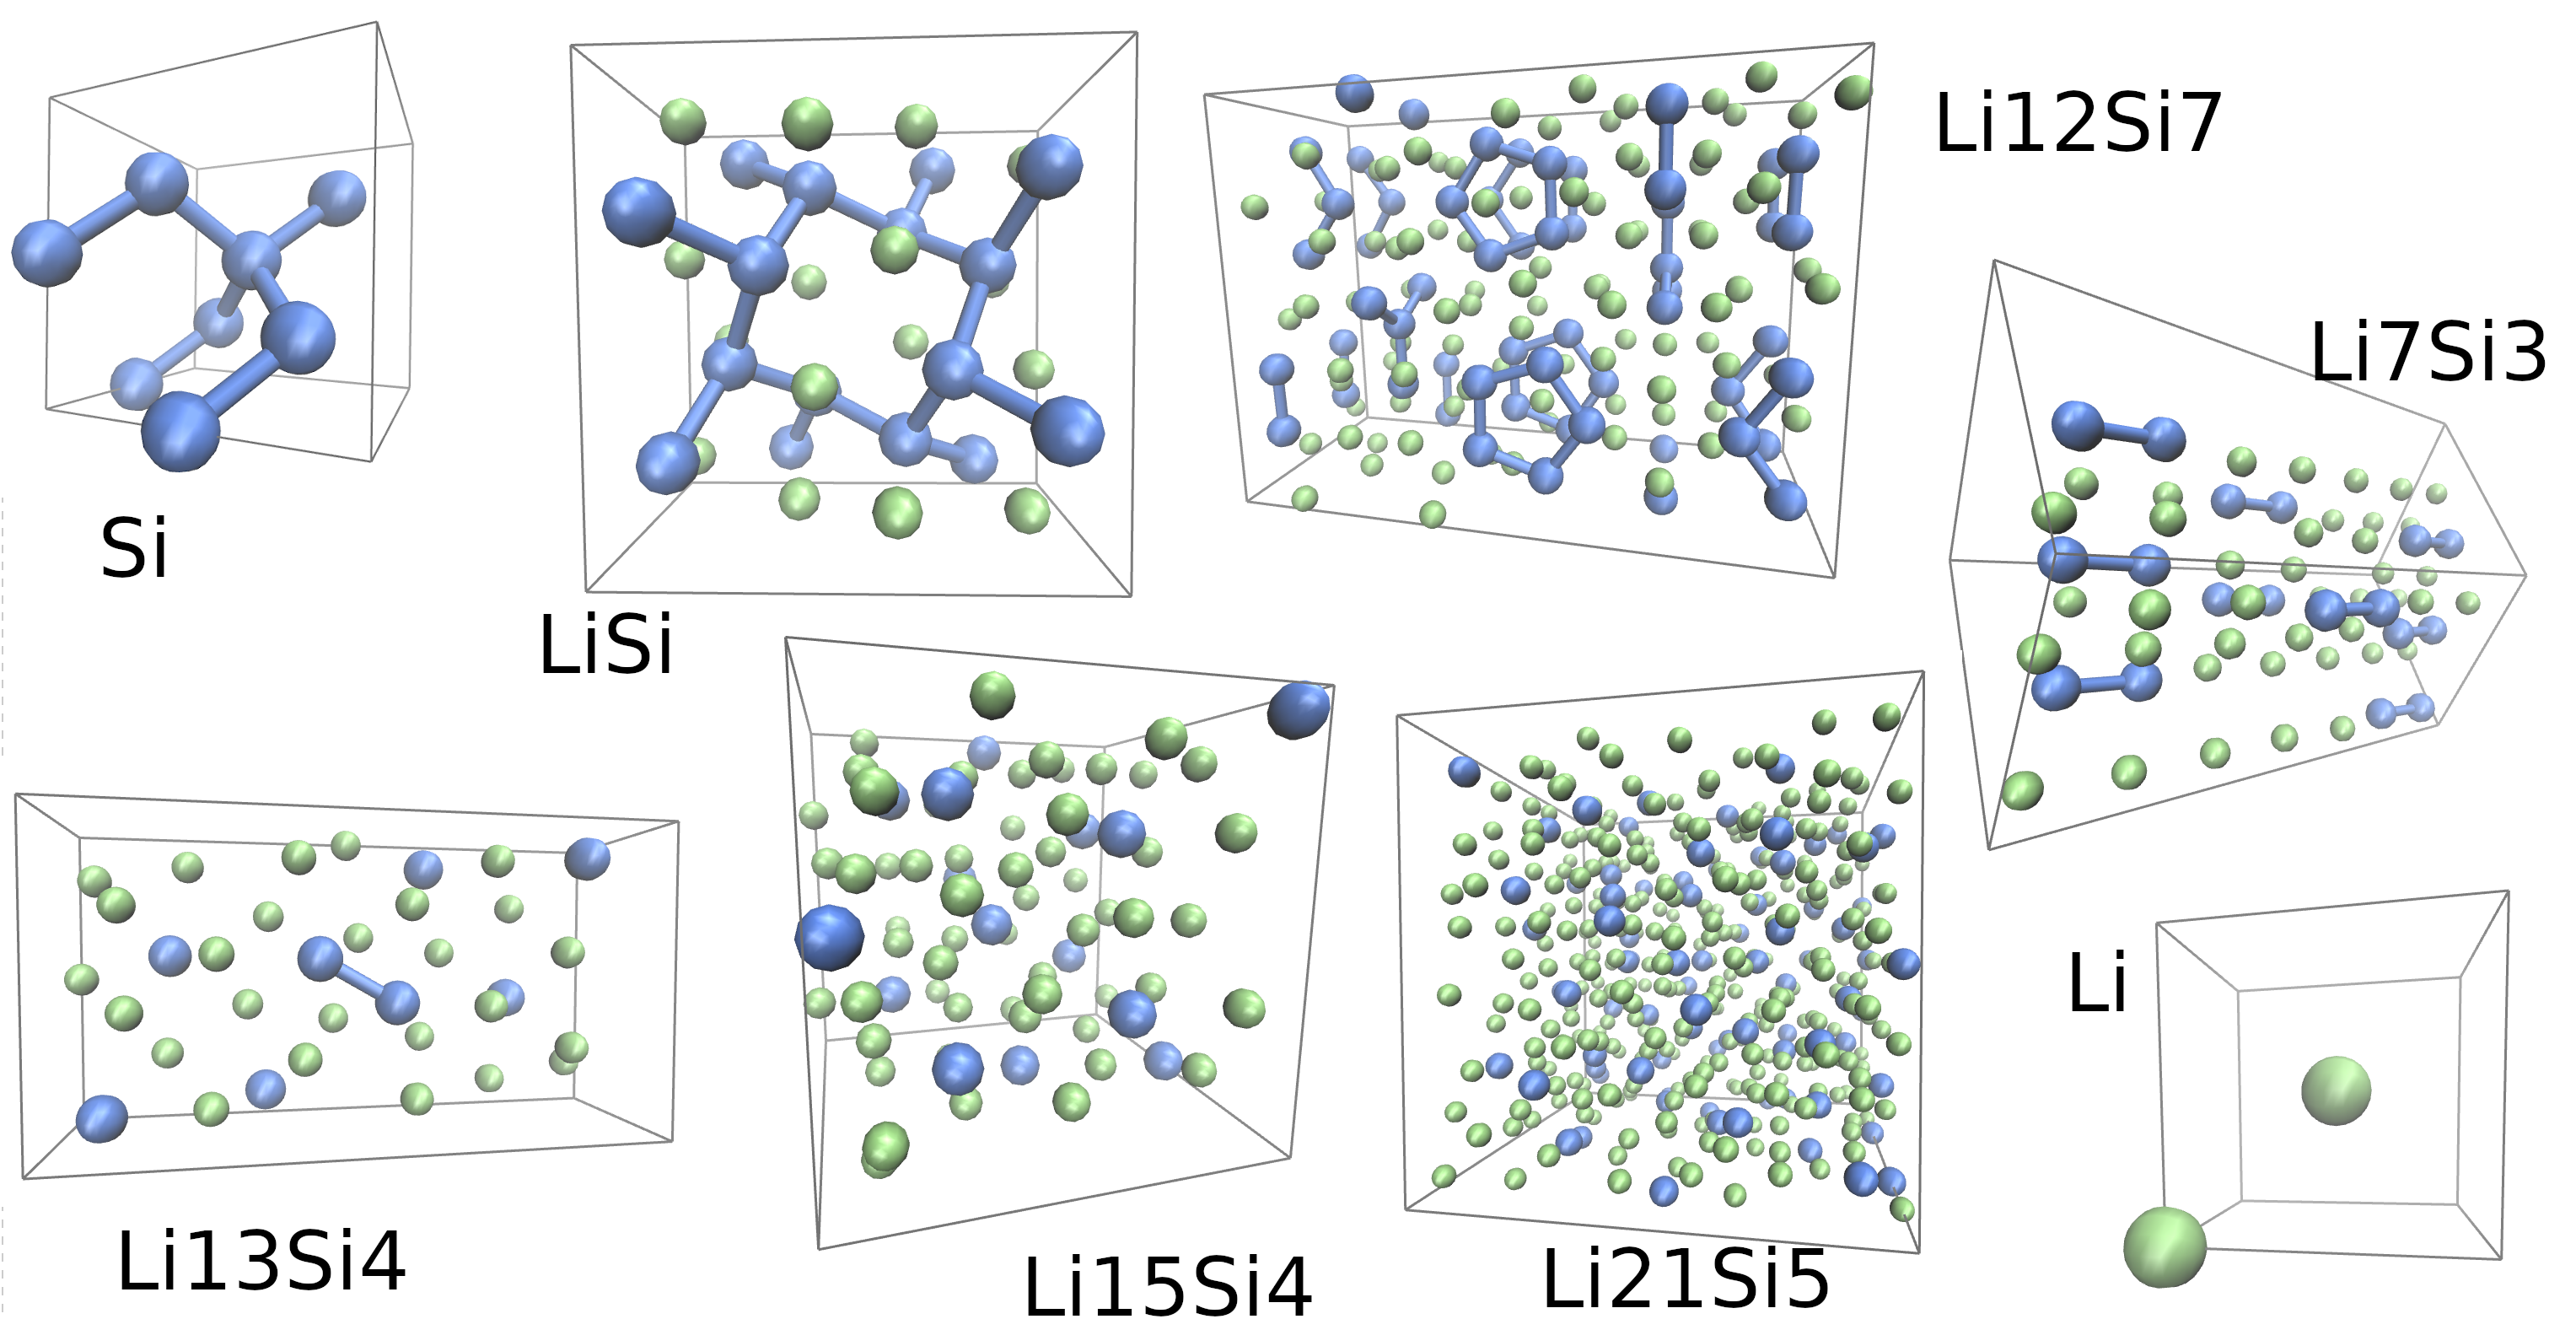
\includegraphics[width=\textwidth]{caracterizacion/cristalinas.png}
    \caption{Estructuras cristalinas de LiSi. Las estructuras no están a escala 
    entre sí. Los átomos de Si se muestran en azul y los de Li en verde, mientras
    que la celda periódica en gris. Los enlaces de Si-Si están graficados si la 
    distancia entre dos de estos átomos es menor a 2.5\AA.}
    \label{fig:cristalinas}
\end{figure}

\subsection{Protocolo de delitiación}

Para obtener configuraciones iniciales para valores de $x$ distintos a los de las 
cristalinas se siguió un protocolo de delitiación en el cual se selecciona la 
estructura cristalina más cercana con un valor de $x$ superior al deseado,
se le extrae un átomo de Li de manera aleatoria y se realiza una dinámica en el 
ensamble NPT durante 2 ps para relajar el volumen. Para estas simulaciones se 
utilizó el termostato de Nosé-Hoover ~\cite{nose1984a, nose1984b, hoover1985} a
300.0 K, un barostato a 0.0 atm y un paso temporal de 1 fs utilizando el
software \path{LAMMPS} ~\cite{lammps1, lammps2}. La extracción del átomo de Li y
la simulación en el ensamble NPT fueron repetidas hasta alcanzar una concentración
deseada. Por último, para algunas concentraciones en particular, se seleccionó la
estructura con la menor presión absoluta como estado inicial para la exploración 
acelerada de mínimos locales que se introduce en la siguiente sección.


\section{Exploración acelerada de mínimos locales}

Las simulaciones de MD tienen un gran poder predictivo para el estudio de 
procesos presentes en las baterías de litio, sin embargo, las escalas de tiempo
están limitadas de unos pocos ns o $\mu$s. El número de operaciones que se 
necesita para alcanzar las escalas de tiempo de la operación de una batería 
experimental son prohibitivos, incluso considerando el uso de potenciales 
semi-empíricos como el ReaxFF en supercomputadoras. Como consecuencia de esto,
la MD usual no es suficiente para una exploración del espacio de las fases y las
estructuras de Li-Si observadas van a estar cercanas a las configuraciones 
iniciales mientras que en el sistema real probablemente pueden aparecer otras
configuraciones. Un método simple y poderoso para acelerar la exploración de 
mínimos locales en sistemas moleculares es el templado simulado 
~\cite{kirkpatrick1983}, en el cual básicamente se busca mejorar la exploración
del espacio de las fases en simulaciones de MD utilizando temperaturas altas y
luego reduciéndola progresivamente hasta encontrar un mínimo de energía a 
temperatura ambiente. El templado simulado múltiple (MSA, de sus siglas en inglés 
\textit{Multiple simluated annealing}) utiliza esta idea en distintas copias del 
sistema y fue utilizado para explorar y encontrar distintas estructuras mínimas 
relevantes cercanas al equilibrio ~\cite{hao2015}.

La presente técnica de simulación, exploración acelerada de mínimos locales (AELM,
de sus siglas en inglés \textit{accelerated exploration of local minima}), es 
similar a la MSA pero en vez de calentar y enfriar lentamente el sistema, se 
utiliza un sesgo en la función de energía potencial para sobrepasar las barrearas
de energía y luego se realiza una minimización local, con algún minimizador local 
como gradientes conjugados o LBFGS, para encontrar el mínimo. Este método permite 
obtener muchas estructuras con energías mínimas relevantes, que son de interés a 
la hora de estudiar electrodos de Li-Si muy ciclados.

Las aleaciones de Li-Si presentan interacciones fuertes entre los átomos que las
conforman, especialmente en el enlace Si-Si donde la energía de enlace es del
orden de $\approx$2 eV ~\cite{wypych2018handbook}. Las barreras de 
energía potencial se espera que sean de ese orden de magnitud, por lo cual un 
muestreo de una MD a temperatura ambiente parece no tener solución. Para explorar 
ampliamente las distintas configuraciones del sistema, $\mathbf{r}$, se 
transforma la superficie de energía potencial (PES, de sus siglas en inglés 
\textit{potencial energy surface}), $V(\mathbf{r})$, usando un potencial sesgado
\begin{equation}\label{eq:bias}
    V_b(\mathbf{r}) = V(\mathbf{r}) + (\alpha - 1) V(\mathbf{r}) = \alpha V(\mathbf{r}),
\end{equation}
donde $\alpha$ es el factor de compresión. El principal efecto de la ecuación 
\ref{eq:bias} es reducir las barreras de la PES, por lo cual el tiempo de
residencia en estados meta-estables es menor que en el sistema sin sesgar y la 
exploración de configuraciones de sistemas diferentes es más eficiente y 
alcanzada en un tiempo de simulación razonable. El término 
$(\alpha - 1) V(\mathbf{r})$ es usualmente referido como la 
\say{función de sesgo}.

La adición de esta función de sesgo a la PES está en la base del método de 
hiper-dinámica (HD), desarrollado por Voter ~\cite{voter1997HD,voter1997method} 
para acelerar la exploración de un sistema sin perder su dinámica. En una 
simulación típica de HD, para recuperar el promedio de alguna propiedad, la 
configuración muestreada son repesadas por un factor $w$ que involucra una función
exponencial y depende del sesgo aplicado. Debido a que este sistema involucra 
cambios grandes en las energías de interacción, comparado con la energía térmica
$k_BT$, lo que implica que la función exponencial en $w$ toma valores muy grandes,
esto provoca que el procedimiento numérico sea inestable y la recuperación de 
la propiedad de interés, como la energía potencial, no sea posible. Ya que este
capítulo se centra en un estudio estructural de los sistemas, podemos descartar
el cálculo del tiempo real evolucionado en la simulación. Además, como el 
funcionamiento de las baterías luego se da a temperatura ambiente, es de esperar
que una vez que se alcanza un mínimo local el sistema explore configuraciones
cercanas a este. Por lo cual se aplica el método de gradientes conjugados (CG)
a cada una de las configuraciones de la HD y de esa forma se muestrea la 
multiplicidad de estructuras.

Este método de exploración introducido en esta tesis se asemeja al templado
simulado, aunque el objetivo es explorar muchas estructuras diferentes en vez de 
encontrar el mínimo global. El templado simulado fue utilizado anteriormente
con este mismo objetivo, Hao \textit{et al.} utilizó la técnica MSA para obtener
distintas estructuras de mínima energía de péptidos ~\cite{hao2015}. En este 
método AELM se usa HD en vez de temperaturas altas para favorecer la exploración,
y se realizan múltiples minimizaciones por CG en vez de simular un enfriado. 


\section{Resultados}

Las simulaciones aceleradas fueron llevadas a cabo en el ensamble NVT a 300.0 K
con un termostato de Langevin ~\cite{schneider1978} utilizando una versión 
modificada de \path{GEMS} ~\cite{gems}. A cada estructura se le realizó una 
minimización de gradientes conjugados con el software \path{LAMMPS} 
~\cite{lammps1, lammps2}. El tamaño de los sistemas y la cantidad de estructuras 
utilizadas para obtener los siguiente resultados se presentan en la tabla 
\ref{t:siminfo}.
\begin{table}[h]
    \centering
    \caption{Información del conjunto de datos.}
    \begin{tabular}{cccccccc}
    \hline
    $x$ en Li$_{x}$Si & N$_{Li}$ & N$_{Si}$ & N$_{estructuras}$ & E$_{mean}$ / N$_T$ [eV] & E$_{std}$ / N$_T$ [eV] & $\sqrt{kT}$ / N$_T$ [eV] \\
    \hline
    0.21 & 140 & 667 & 774 & -4.399 & 0.003 & 0.0002 \\
    0.62 & 416 & 670 & 1665 & -4.002 & 0.005 & 0.0001 \\
    1.25 & 839 & 671 & 1224 & -3.521 & 0.004 & 0.0001 \\
    1.71 & 1152 & 672 & 2132 & -3.286 & 0.002 & 0.0001 \\
    2.17 & 693 & 319 & 1699 & -3.126 & 0.002 & 0.0002 \\
    2.71 & 865 & 319 & 1504 & -2.964 & 0.002 & 0.0001 \\
    3.25 & 1040 & 320 & 1464 & -2.856 & 0.003 & 0.0001 \\
    3.75 & 1080 & 288 & 2660 & -2.777 & 0.002 & 0.0001 \\
    4.20 & 1344 & 320 & 1600 & -2.717 & 0.001 & 0.0001 \\
    \hline
    \end{tabular}
    \label{t:siminfo}
\end{table}

\begin{figure}[th]
    \centering
    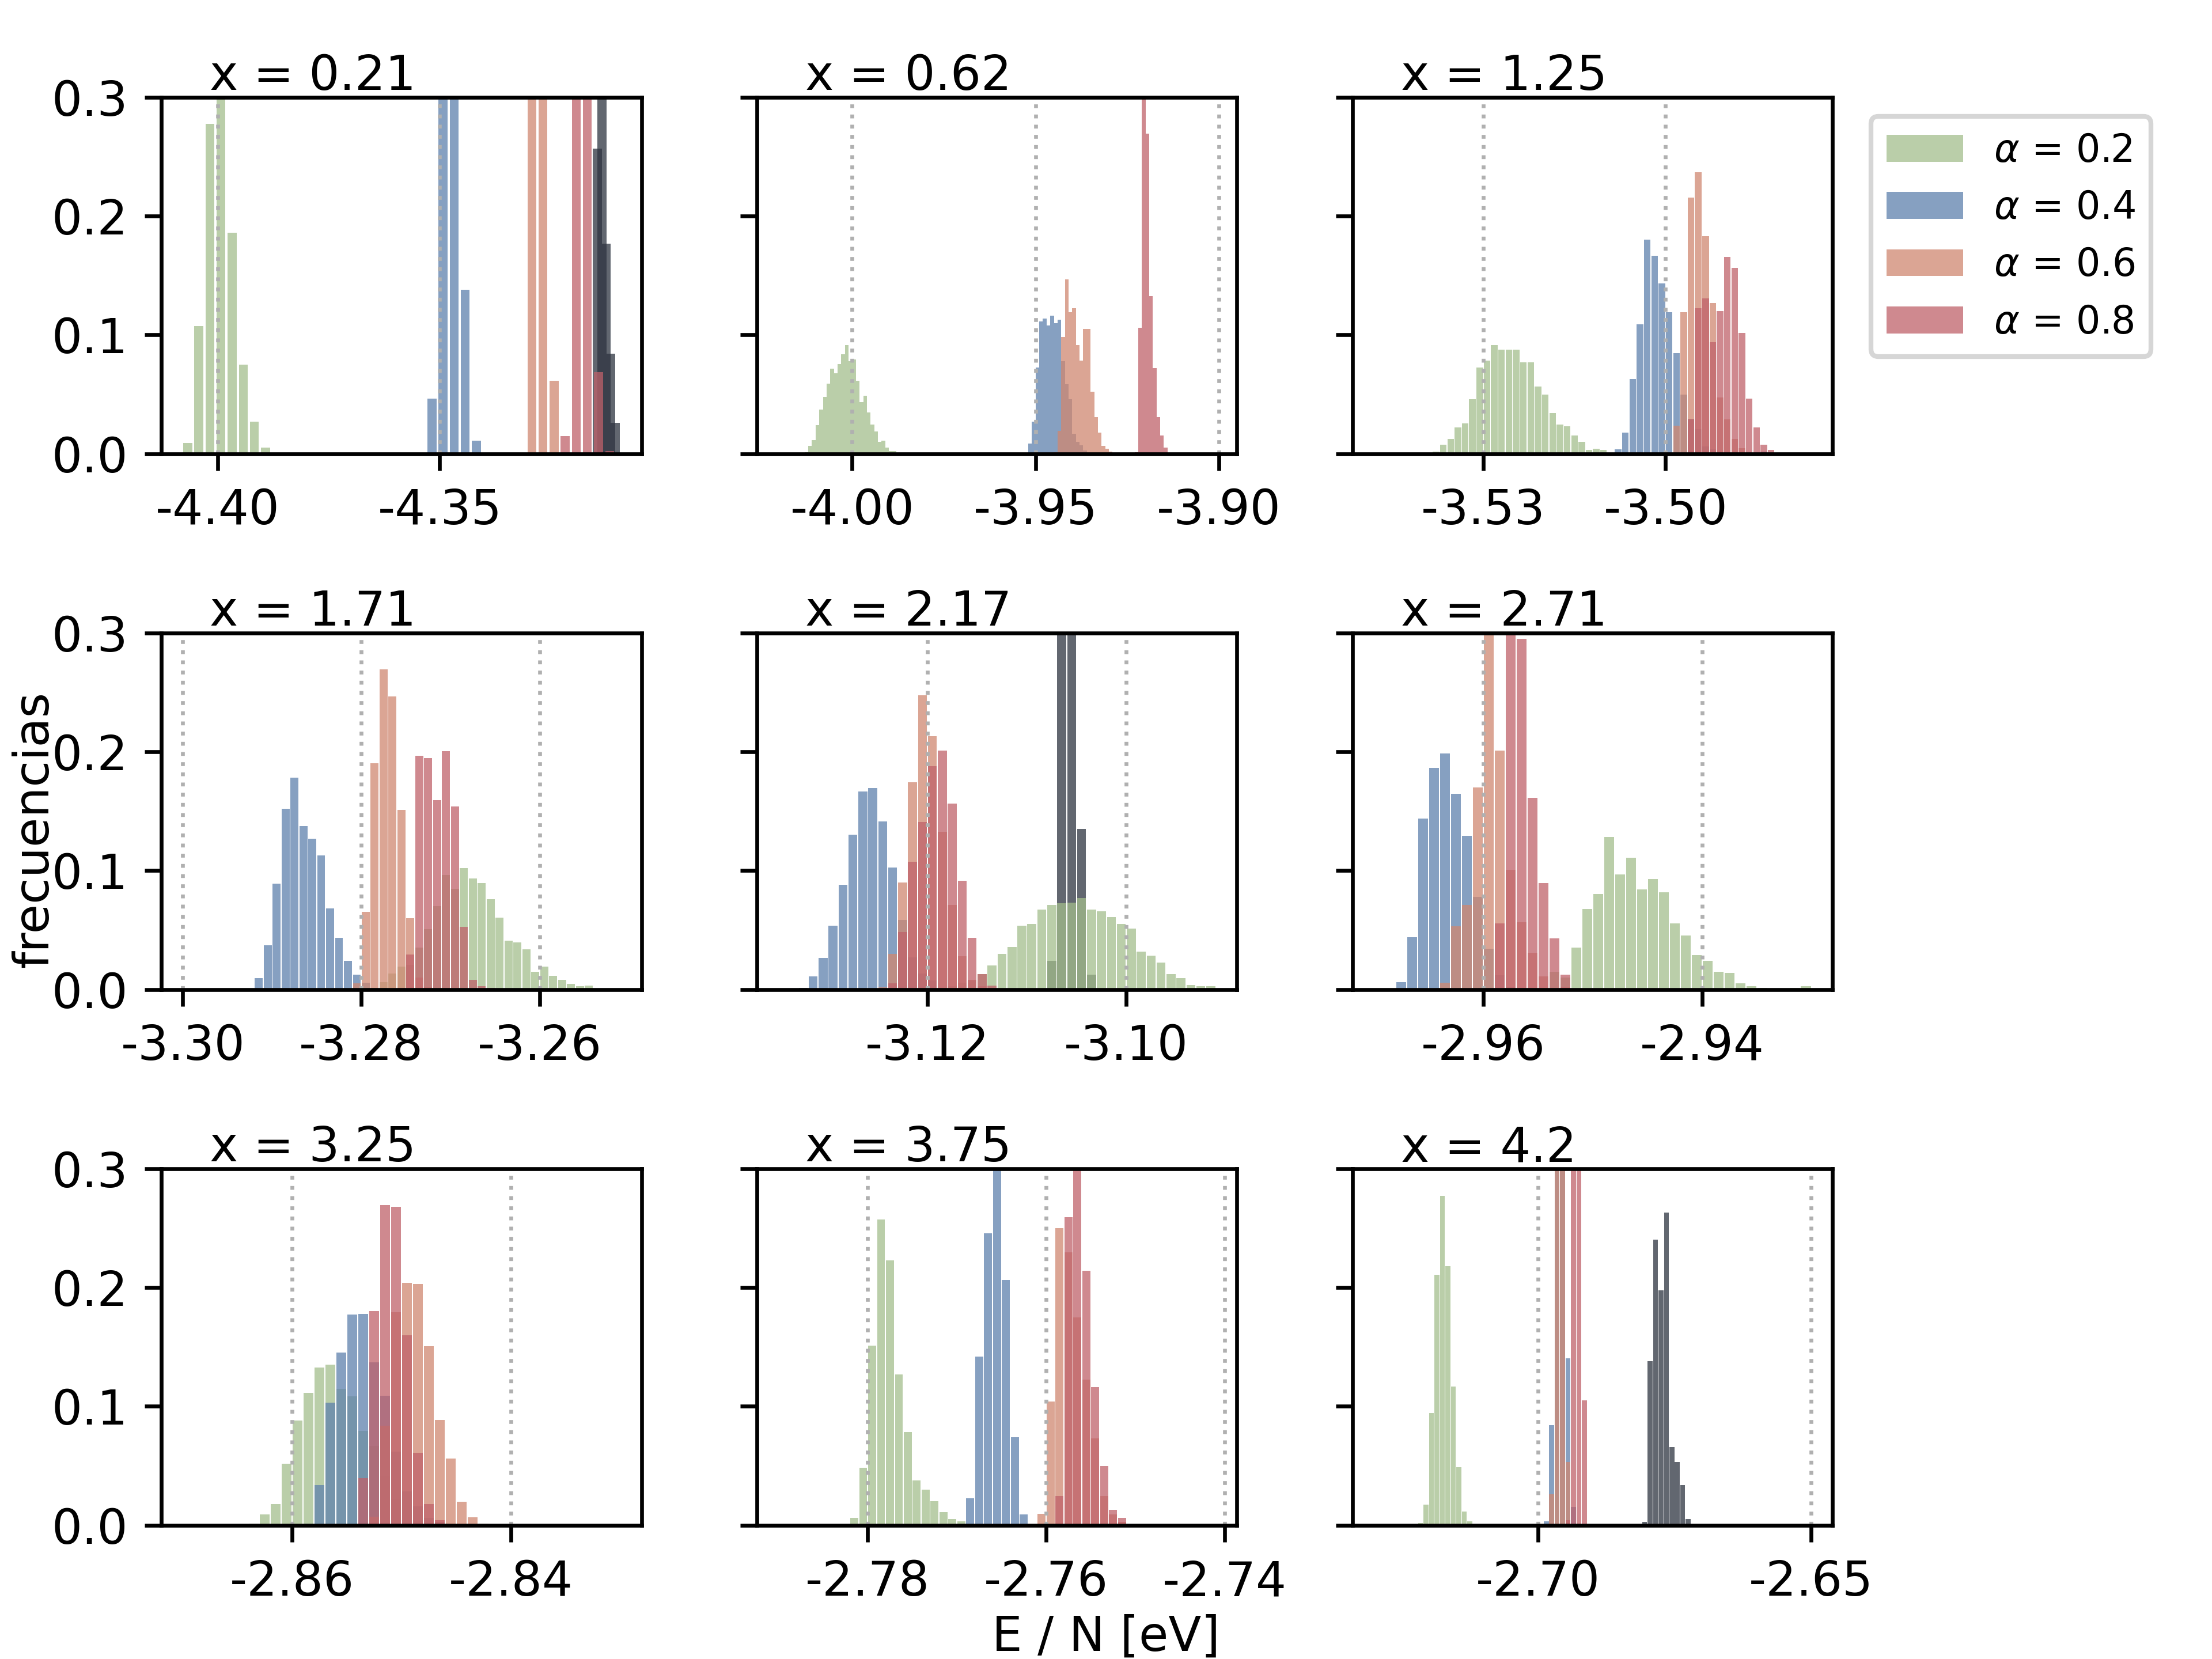
\includegraphics[width=\textwidth]{caracterizacion/energias.png}
    \caption{Histogramas correspondientes a la energía potencial de las 
    estructuras obtenidas con el método AELM, con distintos valores de $\alpha$
    en la ecuación \ref{eq:bias}, para cada composición de Li$_x$Si estudiada.}
    \label{fig:energias}
\end{figure}
La figura \ref{fig:energias} muestra los histogramas para las energías mínimas
de las estructuras de Li$_x$Si obtenidas con el método AELM para los valores de
$x$ estudiados y distintos valores de compresión $\alpha$. En cada fila hay un 
histograma de energías representativo para las estructuras de concentración 
cercana, por lo cual en el análisis sólo son nombradas algunas de estas 
concentraciones. Para el primer caso, donde $x = 0.21$, se puede apreciar como el 
uso de valores más pequeños de $\alpha$ permite que estructuras con menor energía 
sean encontradas. El principal efecto de este factor $\alpha$ sobre la PES es la 
disminución de sus barreras de energía, mejorando la exploración del espacio de 
las fases. Este efecto se vuelve más drástico a medida que el valor de $\alpha$ 
tiende a cero. Para estas concentraciones representativas también se realizaron 
simulaciones de MD usuales, es decir, con un valor de $\alpha = 1$, estas no 
pueden sobrepasar las barreras de energías durante el tiempo simulado. El sistema 
permanece cercano al mínimo local asociado a la configuración inicial. Por otro 
lado, el uso de $\alpha = 0.2$ en el método de AELM resulta en un acceso rápido
a estructuras de energías menores. Un comportamiento similar se observa para 
$x = 2.17$, sin embargo, en este caso el valor más pequeño de $\alpha$ tiende a 
encontrar energías más altas que los otros casos, dando lugar a una distribución
similar a la de MD ordinaria pero con mayores fluctuaciones. Esto probablemente 
se deba a una exploración demasiado extensa, donde el sistema difunde a través
de una gran región del espacio de las fases y las minimizaciones múltiples de 
CG no son capaces de encontrar mínimos de menor energía. Por último, para la 
concentración más alta, correspondiente a un valor de $x = 4.2$, las simulaciones 
de AELM con un valor de $\alpha = 0.2$ son capaces de encontrar estructuras que 
reducen fuertemente la energía potencial del sistema. 

\begin{figure}[t]
    \centering
    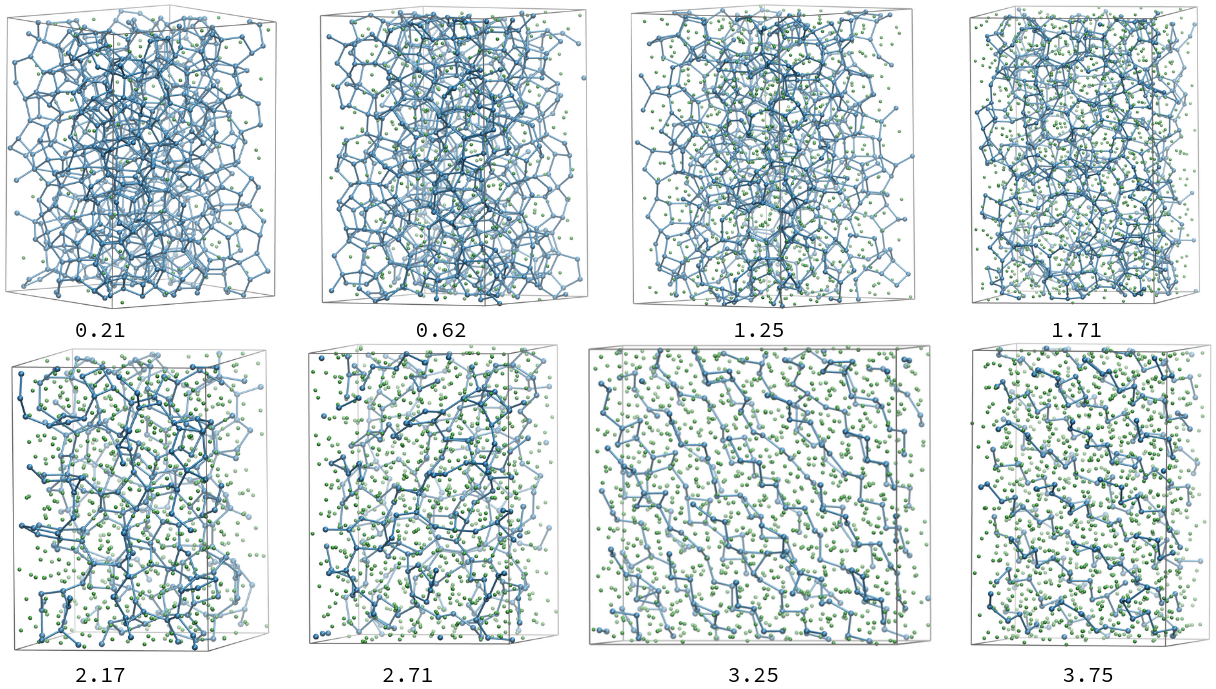
\includegraphics[width=\textwidth]{caracterizacion/amorfas.png}
    \caption{Configuración amorfa representativa de cada valor de $x$. Los átomos
    de Si se muestran en azul mientras que los de Li en verde.}
    \label{fig:amorfas}
\end{figure}
De los histogramas de la figura \ref{fig:energias} se seleccionan los factores 
de aceleración más óptimos, es decir que producen energías menores, para obtener
las propiedades estructurales que se discuten a continuación. Para estos valores
se muestra una estructura representativa a cada composición en la figura 
\ref{fig:amorfas}. Para $x = 0.21$ puede verse que la red amorfa de silicio
permanece con su estructura tetraédrica desordenada. Algunos enlaces Si-Si 
comienzan a romperse a medida que la concentración de litio aumenta, como puede
verse para las estructuras cercanas a $x = 2.17$. Por último, para las 
concentraciones más altas de litio, se alcanzan estructuras que involucran 
cadenas unidimensionales periódicas de silicio. Una estructura similar ha sido 
reportada por Ostadhossein \textit{et al.} ~\cite{ostadhossein2015}. En las 
próximas secciones se caracterizan dichas estructuras.

\subsection{Comportamiento electroquímico}

\subsubsection{Cambio de volumen fraccionario}

El cambio de volumen fraccionario puede definirse utilizando una normalización 
relativa al número de átomos de Si en la estructura de acuerdo a
\begin{equation}\label{eq:fvc}
    fvc = \frac{N_{Si}}{V_{Si}} \left( \frac{V_{Si,x}}{N_{Si,x}} - \frac{V_{Si}}{N_{Si}} \right),
\end{equation}
donde $V_{Si}$ y $N_{Si}$ son el volumen y el número de átomos de Si en la celda
unidad de c-Si, $V_{Si,x}$ y $N_{Si,x}$ son el volumen y el número de átomos de Si
en la celda de simulación para el valor correspondiente de $x$. En la figura
\ref{fig:fvc} se muestran los valores calculados a partir de la ecuación 
\ref{eq:fvc} para las distintas estructuras de Li$_x$Si estudiadas. En la misma 
se comparan los valores obtenidos con datos experimentales de AFM (\textit{atomic 
force microscopy}, sus siglas en inglés) medidos por Beaulieu \textit{et al.} 
~\cite{beaulieu2003} y con predicciones de DFT con un cambio volumétrico fijo 
utilizado por Chevrier y Dahn ~\cite{chevrier2009}. Los mismos muestran que el
potencial ReaxFF proporciona una tendencia correcta tanto cualitativa como 
cuantitativamente.
\begin{figure}[th]
    \centering
    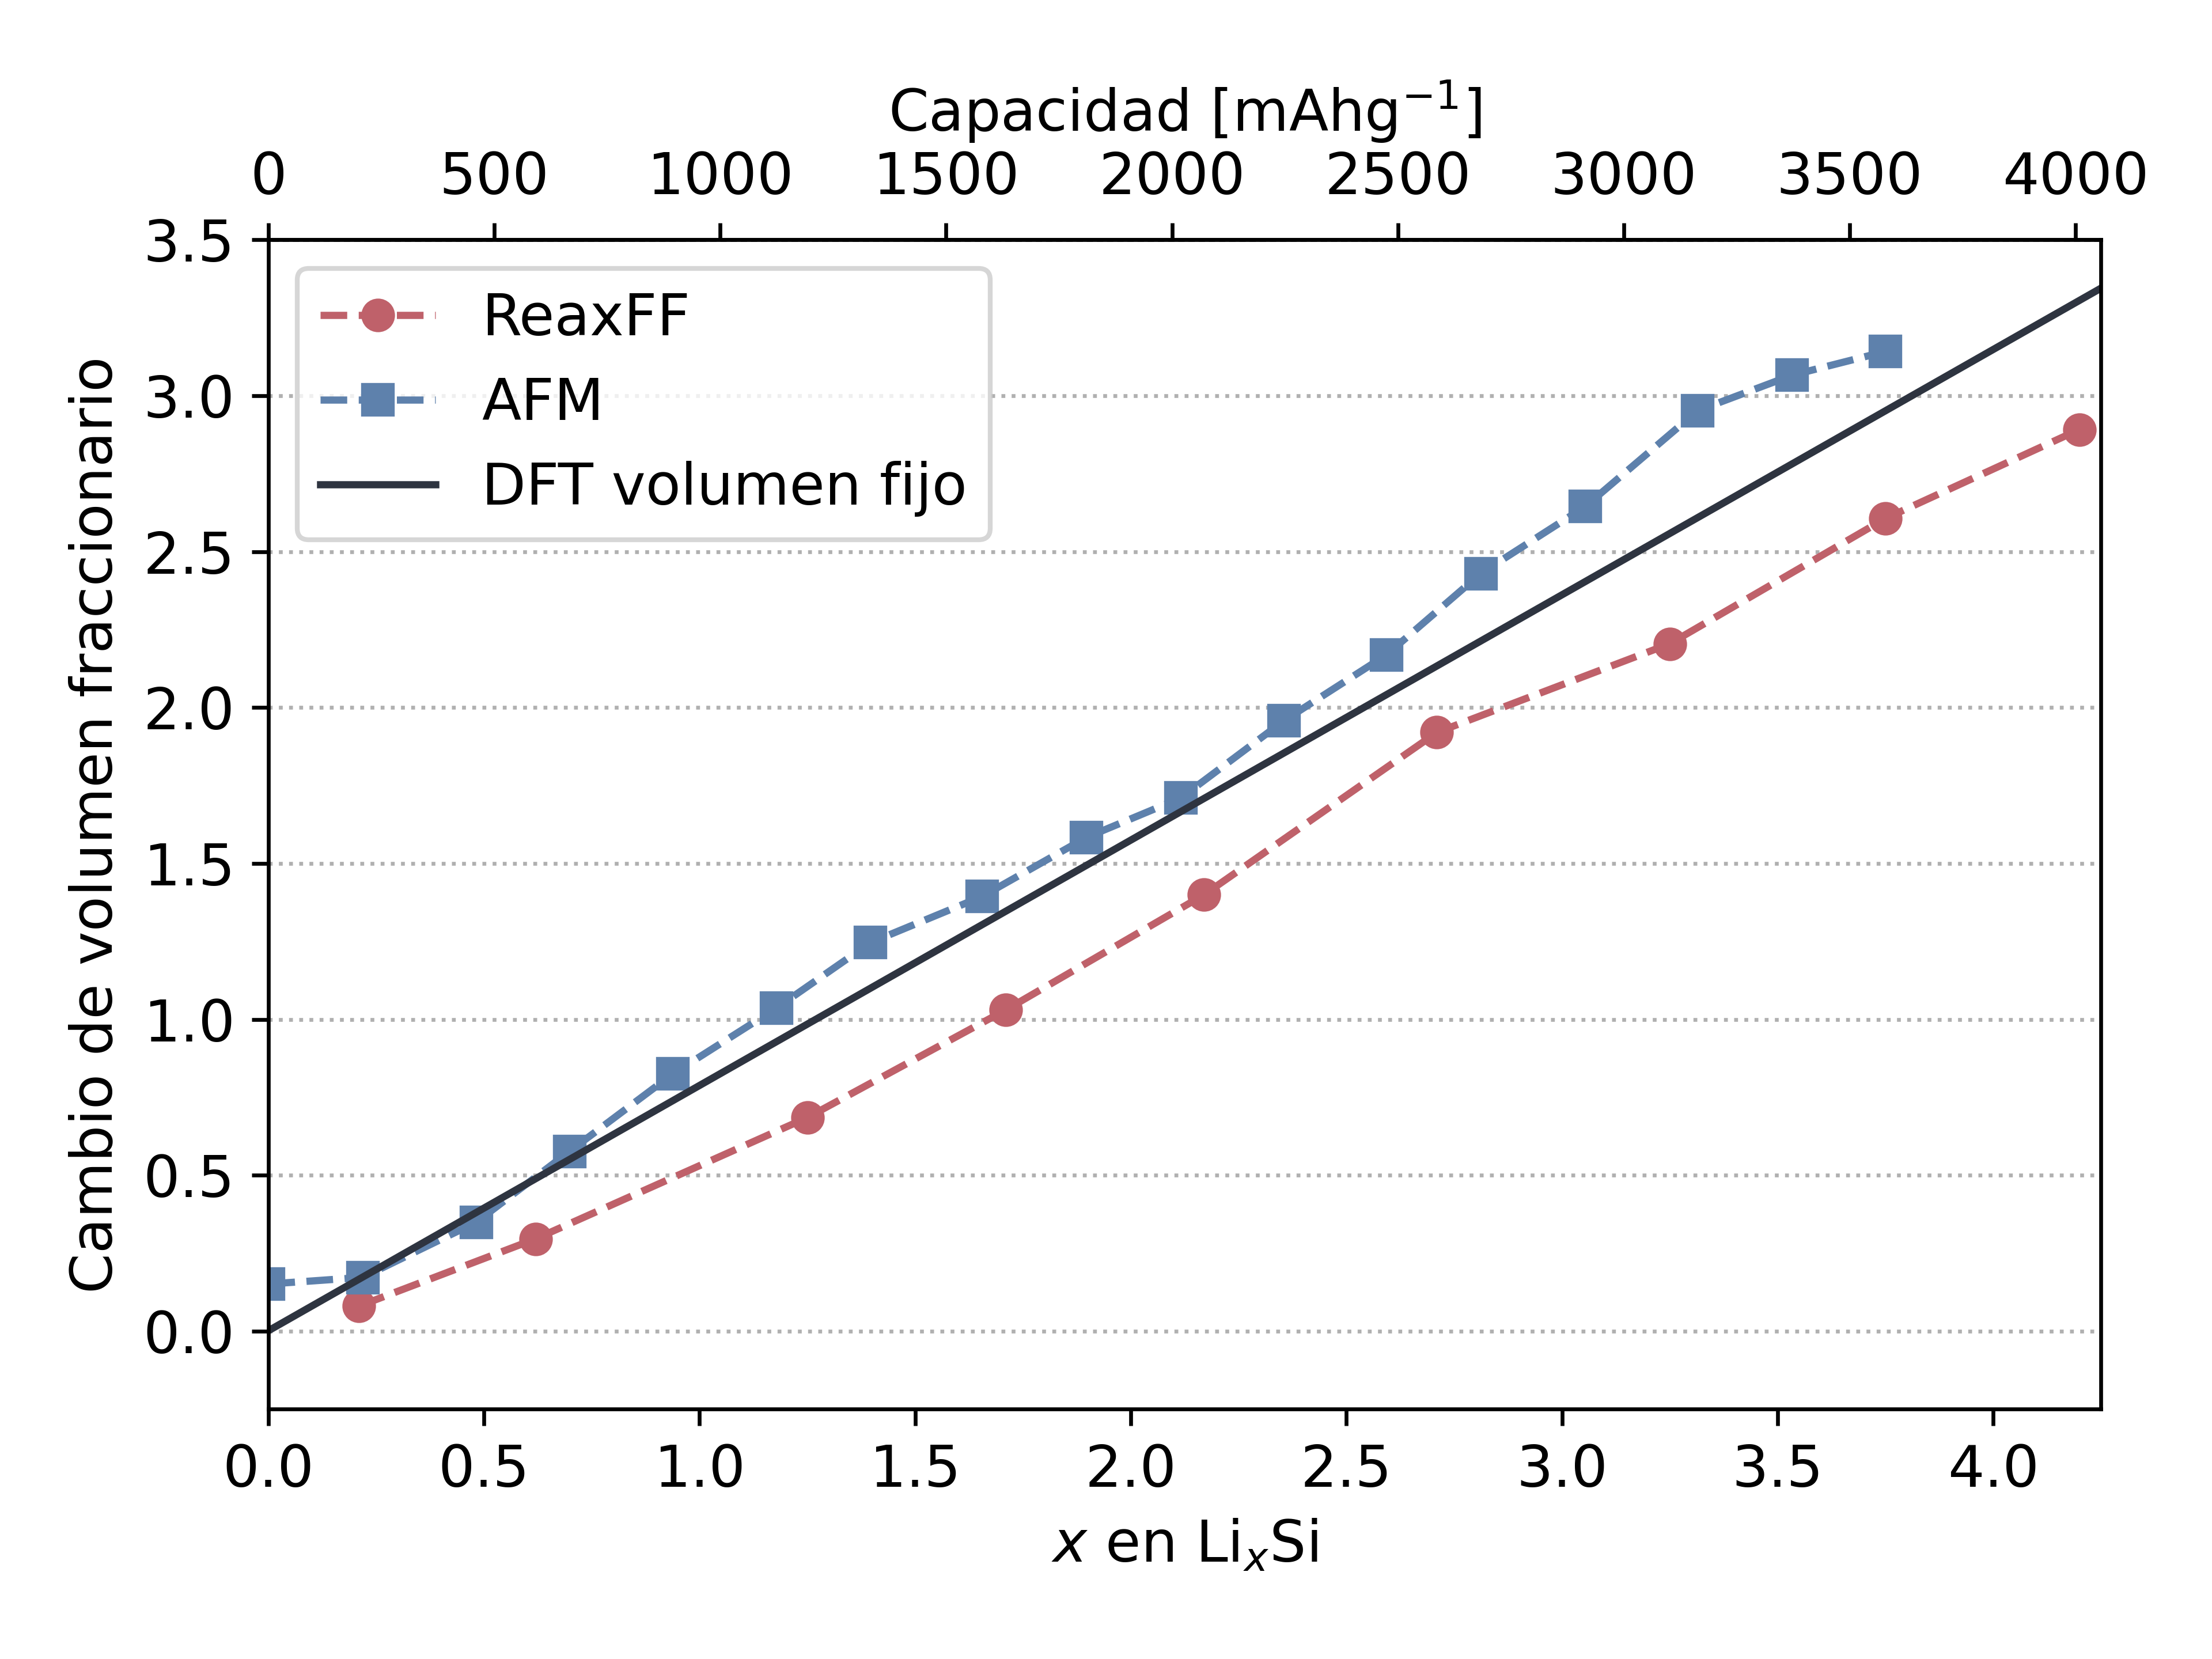
\includegraphics[width=0.8\textwidth]{caracterizacion/fvc.png}
    \caption{Cambio de volumen fraccionario en función de la composición de la 
    aleación. Los valores experimentales de AFM se muestran con cuadrados azules, 
    la línea recta se corresponde con cálculos de DFT y los círculos rojos son 
    resultados de este trabajo.}
    \label{fig:fvc}
\end{figure}

\subsubsection{Voltaje}

\begin{table}[h]
    \centering
    \caption{Energías de formación obtenidas a través de la ecuación \ref{eq:fe}}
    \begin{tabular}{ccc}
    \hline
    x en Li$_x$Si & Energía de formación [eV] & Desviación estándar [eV]\\
    \hline
    0.21  &  0.5027  &  0.0037 \\
    0.62  &  0.1206  &  0.0074 \\
    1.25  & -0.1160  &  0.0096 \\
    1.71  & -0.2358  &  0.0065 \\
    2.17  & -0.3551  &  0.0075 \\
    2.71  & -0.4098  &  0.0072 \\
    3.25  & -0.5187  &  0.0126 \\
    3.75  & -0.6202  &  0.0097 \\
    4.20  & -0.6995  &  0.0075 \\
    \hline
    \end{tabular}
    \label{t:fe}
\end{table}
Las energías obtenidas pueden ser utilizadas para testear el funcionamiento del 
modelo para predecir propiedades electroquímicas, como fue sugerido por Chevrier
y Dahn ~\cite{chevrier2009}. Primero, se define la energía de formación de las 
distintas estructuras amorfas como
\begin{equation}\label{eq:fe}
    E_f(x) = E_{Li_xSi} - (x E_{Li} + E_{Si}),
\end{equation}
donde $E_{Li_xSi}$ es la energía de la aleación Li$_x$Si por átomo de Si, E$_{Li}$
y E$_{Si}$ son las energías cohesivas de Li y Si en sus fases cristalinas. Usando
la ecuación \ref{eq:fe} como aproximación a la energía de formación de Gibbs, el 
potencial \textit{versus} Li metálico de Li$_x$Si puede obtenerse a partir de
\begin{equation}\label{eq:voltaje}
    V(x) = - \frac{dE_f(x)}{dx},
\end{equation}
donde $V$ es el potencial. Los datos obtenidos así pueden compararse con valores
experimentales y computacionales previos. Las energías de formación calculadas
a partir de la ecuación \ref{eq:fe} se muestran en la tabla \ref{t:fe}. 
Realizándoles un \textit{spline} a estos valores, mostrados en el recuadro de la
figura \ref{fig:voltaje}, los valores de $V(x)$ son obtenidos de la ecuación
\ref{eq:voltaje} y son graficados en función de la composición en la figura 
\ref{fig:voltaje} con una línea roja. Para comparar, se incluye en la misma figura
las curvas experimentales medidas para la litiación y la delitiación de silicio
amorfo ~\cite{hatchard2004} y la curva teórica de cálculos de primeros principios 
~\cite{chevrier2009}. Se puede afirmar que los resultados obtenidos con el ReaxFF 
son bastante satisfactorios.
\begin{figure}[th]
    \centering
    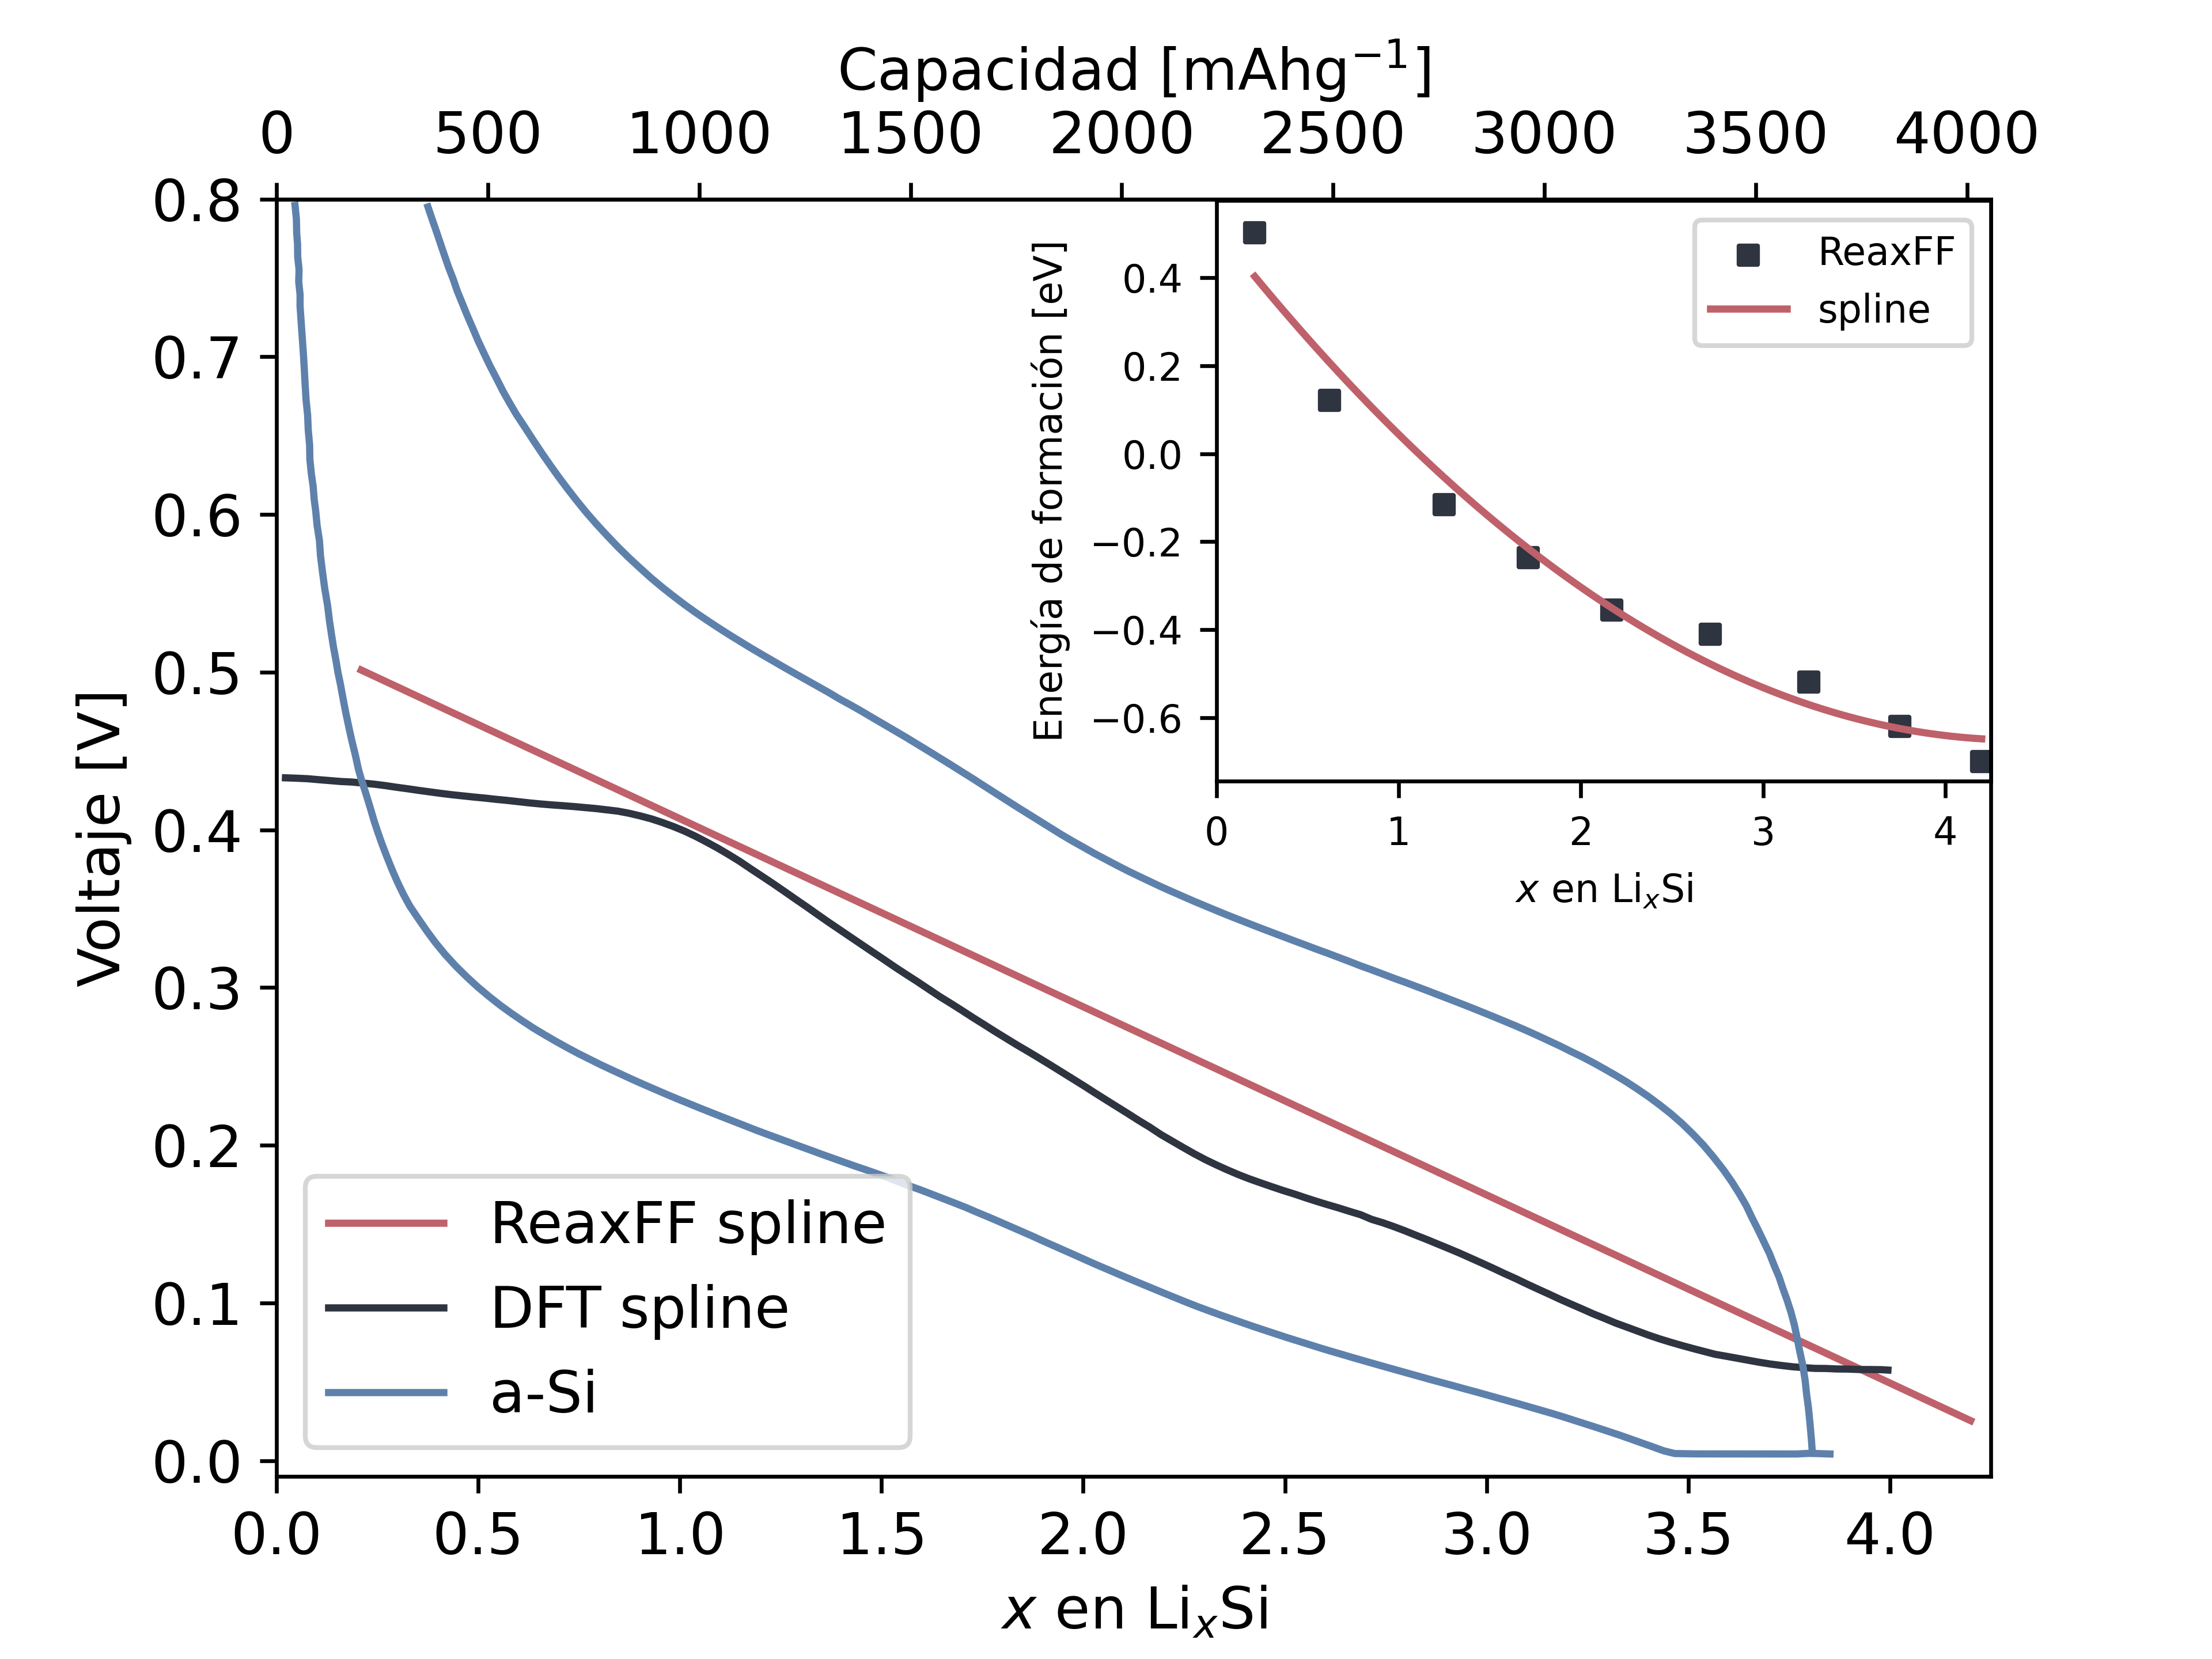
\includegraphics[width=0.8\textwidth]{caracterizacion/voltaje.png}
    \caption{Curvas potencial-concentración de la litiación de ánodos de Si.
    La línea negra se corresponde con cálculos de DFT, las líneas azules con 
    curvas medidas experimentalmente en la litiación de Si amorfo y la línea 
    roja es la derivada del \textit{spline} ajustado a los datos de la energía 
    de formación obtenidos con el ReaxFF, presentados en el recuadro.}
    \label{fig:voltaje}
\end{figure}

\subsection{Distribución radial de a pares}

La distribución radial de a pares, introducida en la sección \ref{s:observables},
puede ser utilizada para describir la estructura de materiales amorfos. Para el 
caso de sistemas que están conformados por más de un elemento se pueden analizar 
las distribuciones radiales de a pares parciales ~\cite{lamparter1995}, donde la 
$g_{ij}(r)$ representa la RDF de los átomos $j$ a una distancia $r$ alrededor de 
los átomos centrales $i$, y que es lo mismo que considerar $g_{ji}(r)$. Las 
figuras \ref{fig:rdf-LiLi}, \ref{fig:rdf-SiSi}, \ref{fig:rdf-SiLi} muestran los
resultados obtenidos para las RDF de Li-Li, Si-Si y Si-Li, respectivamente. En
cada una de ellas se analizan los cambios en la estructura que se dan para los
distintos valores de $x$ en Li$_x$Si estudiados, las curvas se calculan sobre los
\textit{frames} minimizados de la HD.

\begin{figure}[h!]
    \centering
    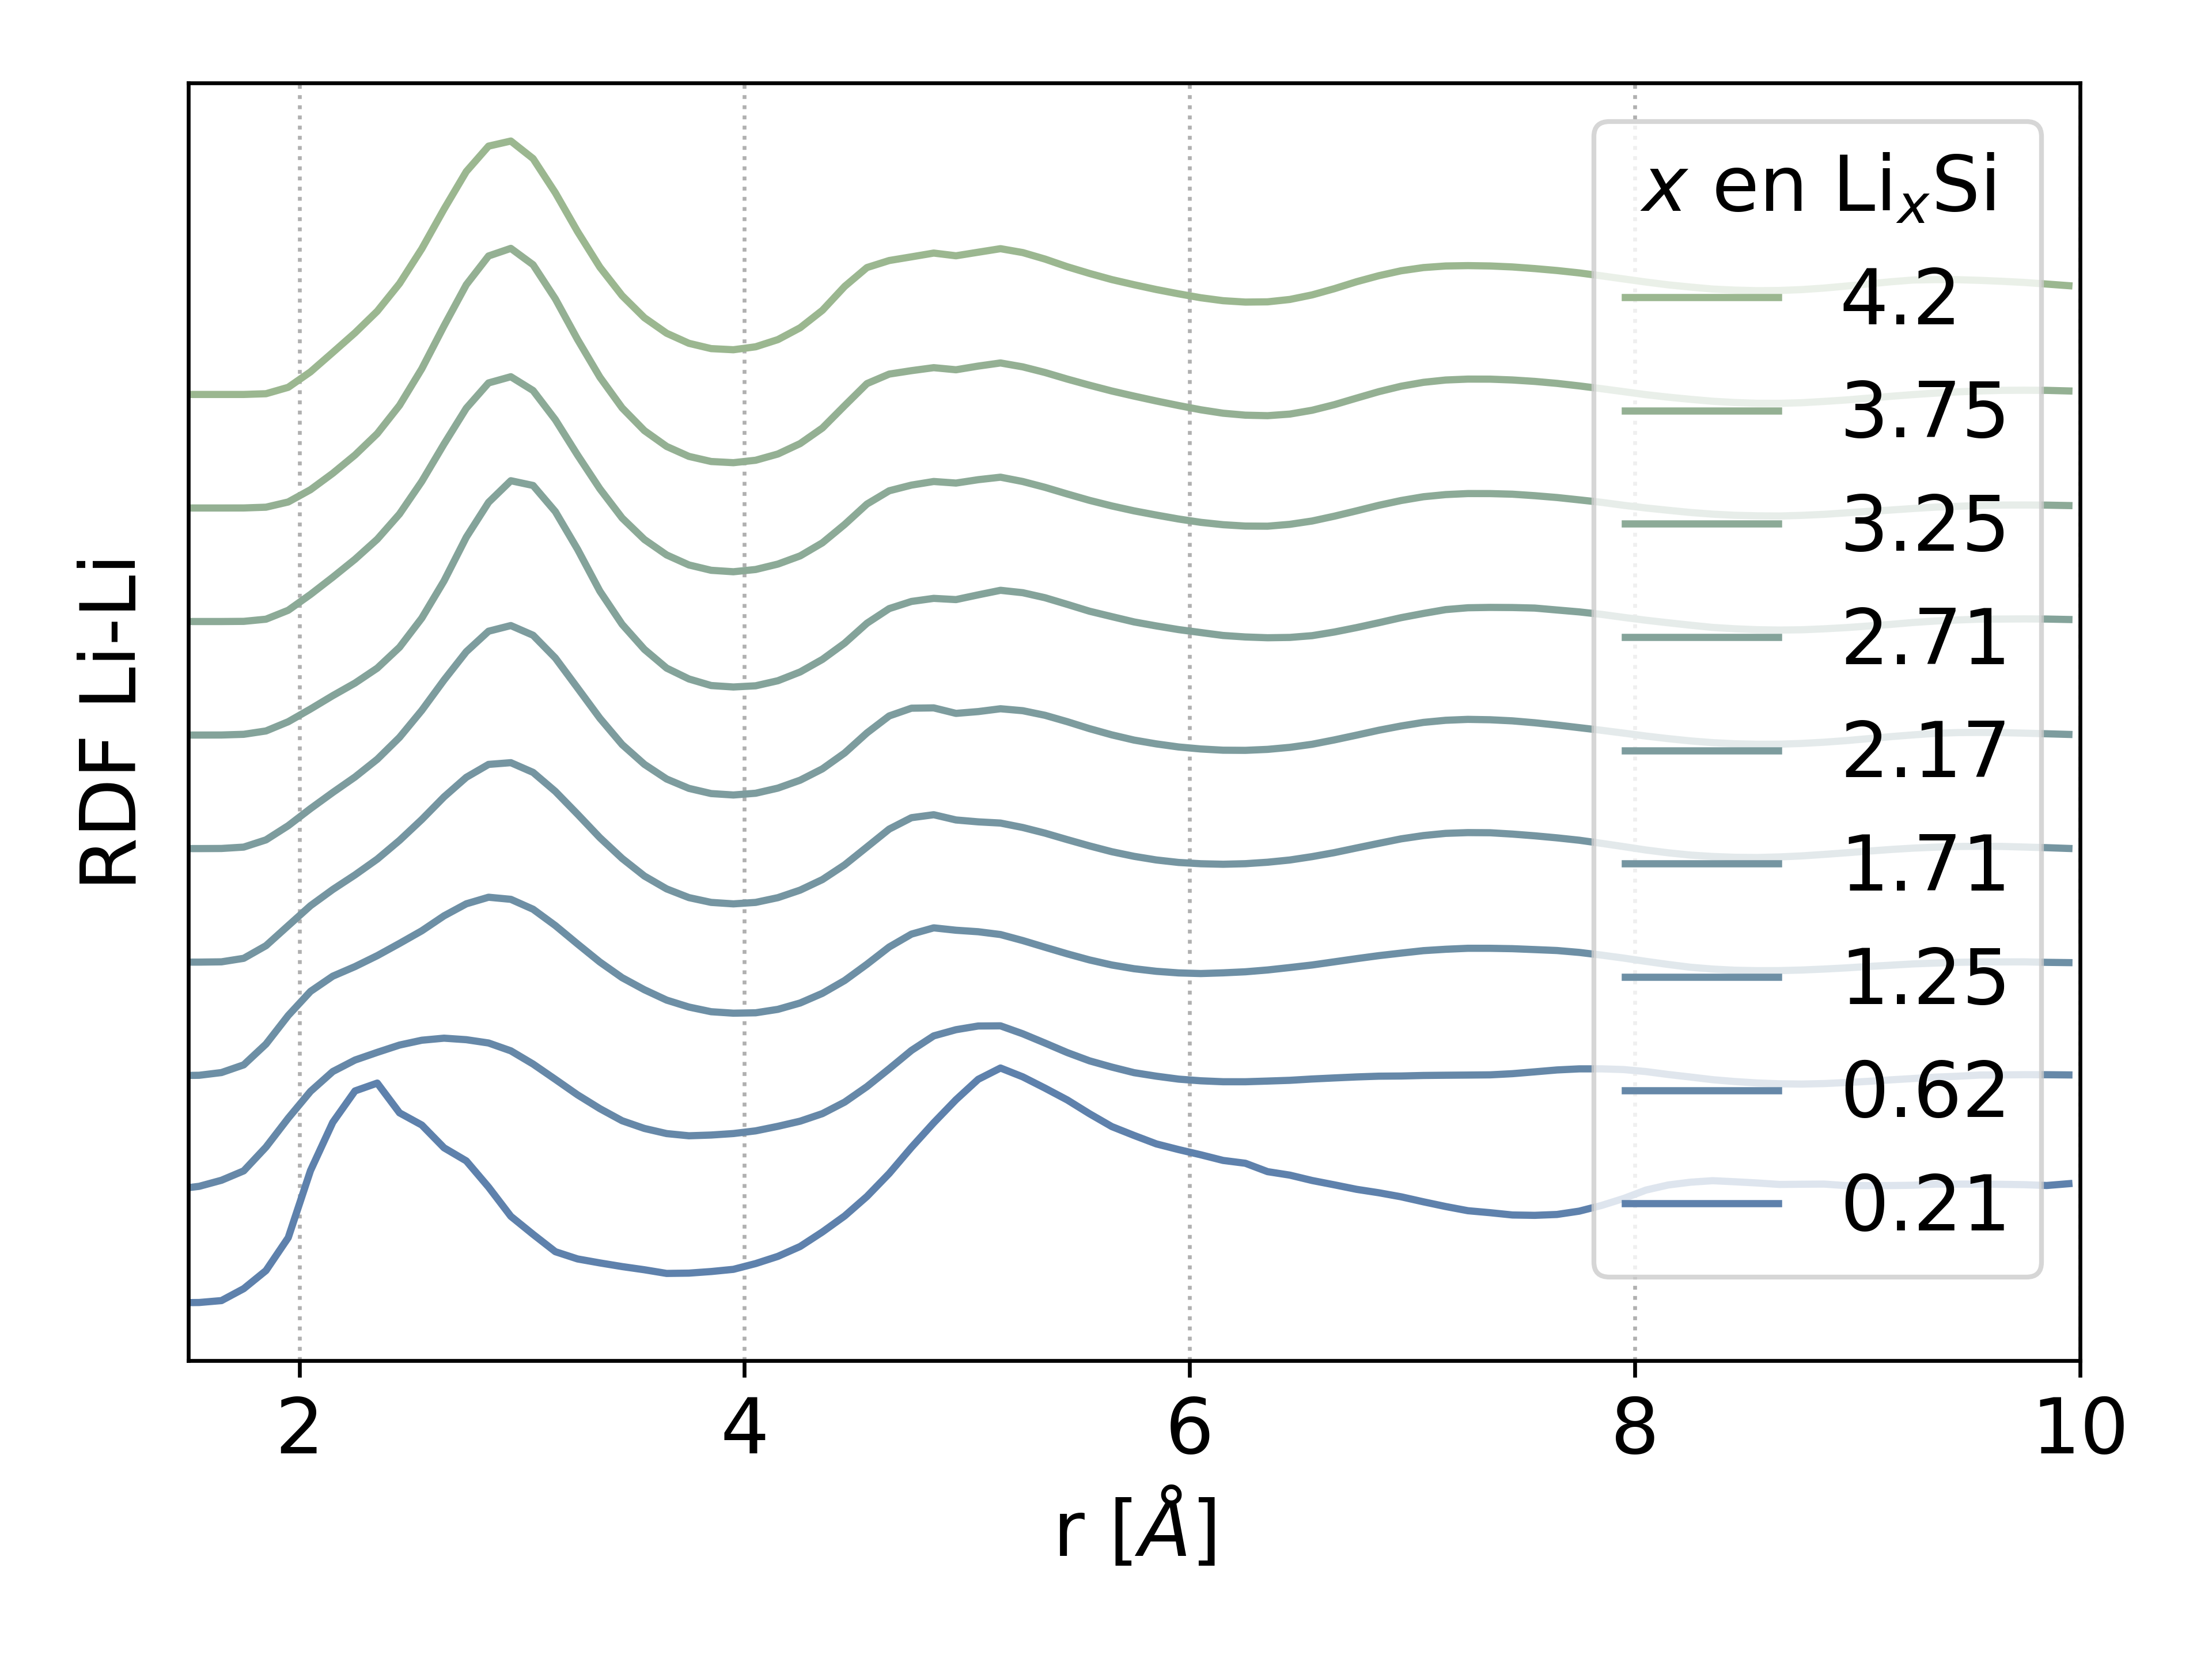
\includegraphics[width=0.8\textwidth]{caracterizacion/rdf-LiLi.png}
    \caption{Distribución radial de a pares para Li-Li de las estructuras 
    minimizadas. Cada curva se corresponde con un valor de concentración 
    distinto.}
    \label{fig:rdf-LiLi}
\end{figure}
Lo más relevante a destacar de la RDF$_{Li-Li}$ es que su primer pico comienza 
centrado en 2.45 \AA\ para las concentraciones de iones de Li más bajas y que 
luego dicho pico aumenta su posición a distancias más grandes a medida que aumenta 
$x$ hasta permanecer en 2.95 \AA\ para $x$ mayores a 1.71. La altura de este pico
aumenta en un 50\% luego de la litiación completa, relativa a la menor 
concentración.

\begin{figure}[h!]
    \centering
    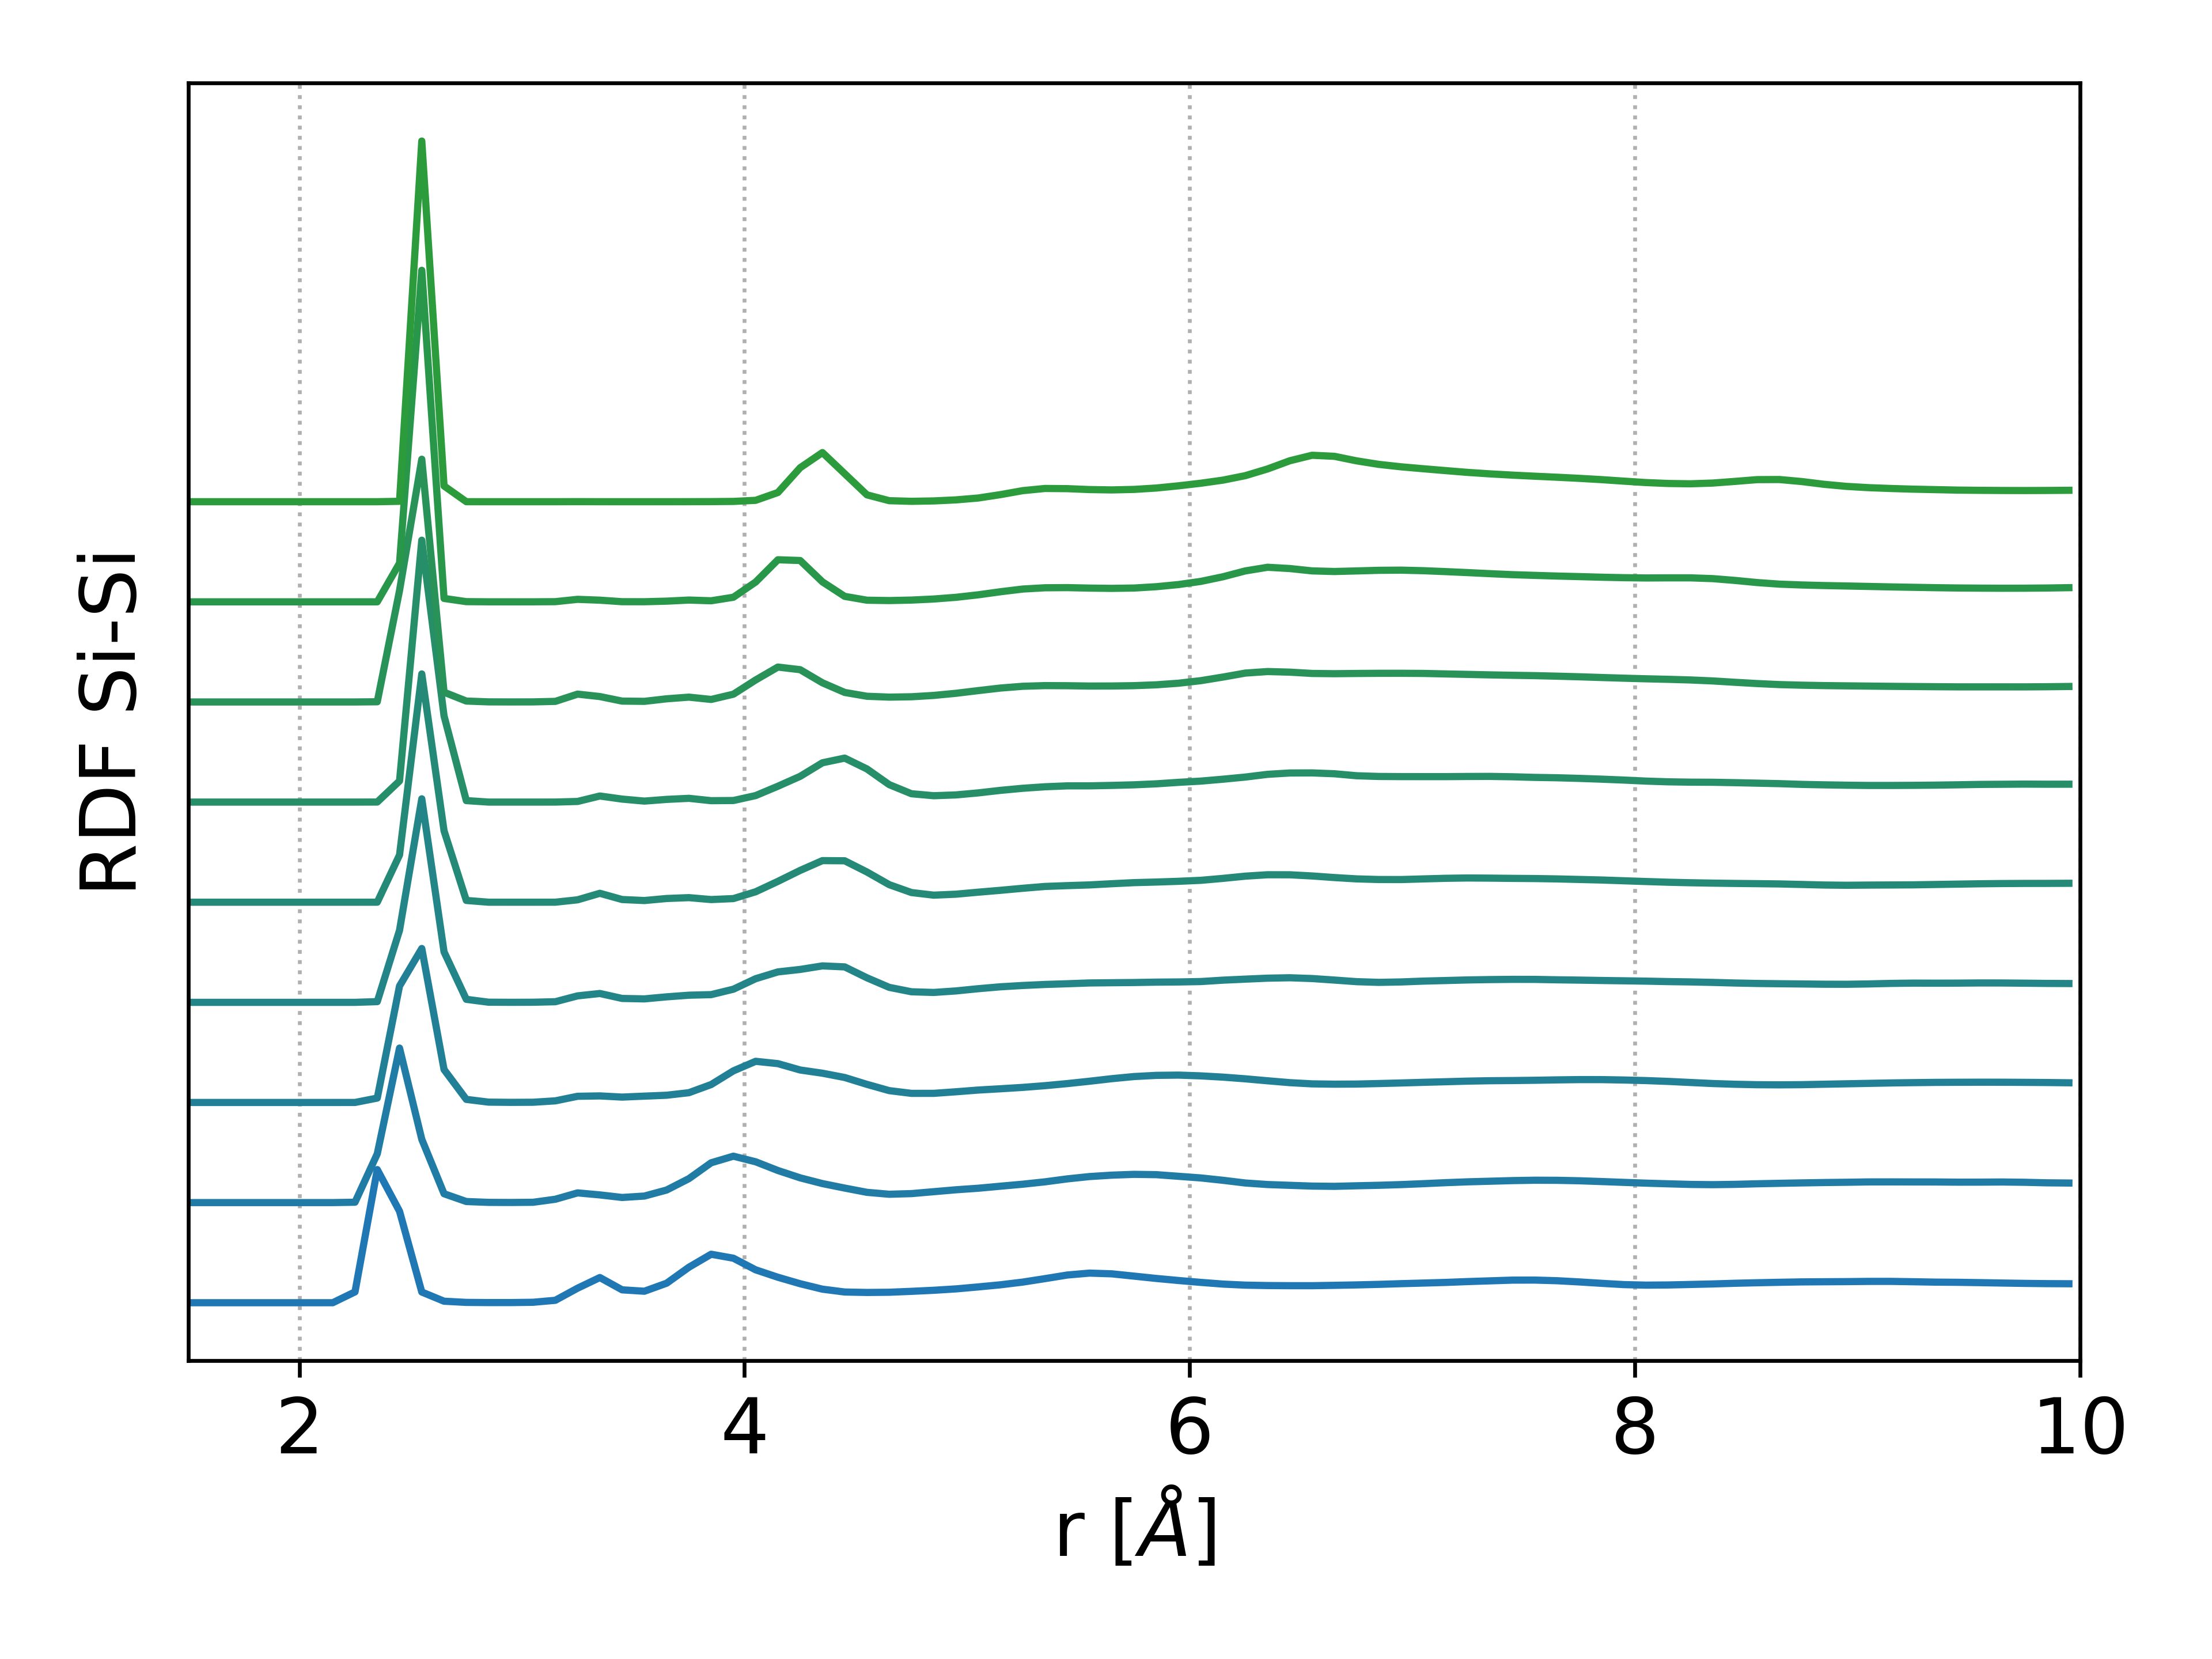
\includegraphics[width=0.8\textwidth]{caracterizacion/rdf-SiSi.png}
    \caption{Distribución radial de a pares para Si-Si de las estructuras 
    minimizadas. Cada curva se corresponde con un valor de concentración 
    distinto.}
    \label{fig:rdf-SiSi}
\end{figure}
Este mismo efecto se ve en el primer pico de la RDF$_{Si-Si}$, el centro del mismo
se encuentra en 2.4 \AA\ para $x = 0.21$ y luego se desplaza a distancias
mayores, después de $x = 1.25$ el centro se encuentra entre 2.52 y 2.56 \AA.
Mientras que la altura del pico aumenta se ve un decrecimiento en en el ancho 
del pico, el valor del FWHM va de 0.14 \AA\ a 0.05 \AA\ para $x = 0.21$ y 
$x = 3.75$, respectivamente. Por otro lado, el segundo pico de la RDF$_{Si-Si}$
también se desplaza hacia distancias mayores, se divide en dos picos para valores 
de $x$ entre 0.62 y 1.71 y vuelve a comportarse como un sólo pico para para 
concentraciones mayores. Entre el primer y el segundo pico se observa un hombro,
como señaló previamente Fan \textit{et al.} ~\cite{fan2013}. Los resultados 
obtenidos para la RDF$_{Si-Si}$ están en concordancia con las mediciones 
experimentales reportadas por Key \textit{et al.} ~\cite{key2011}.

\begin{figure}[h!]
    \centering
    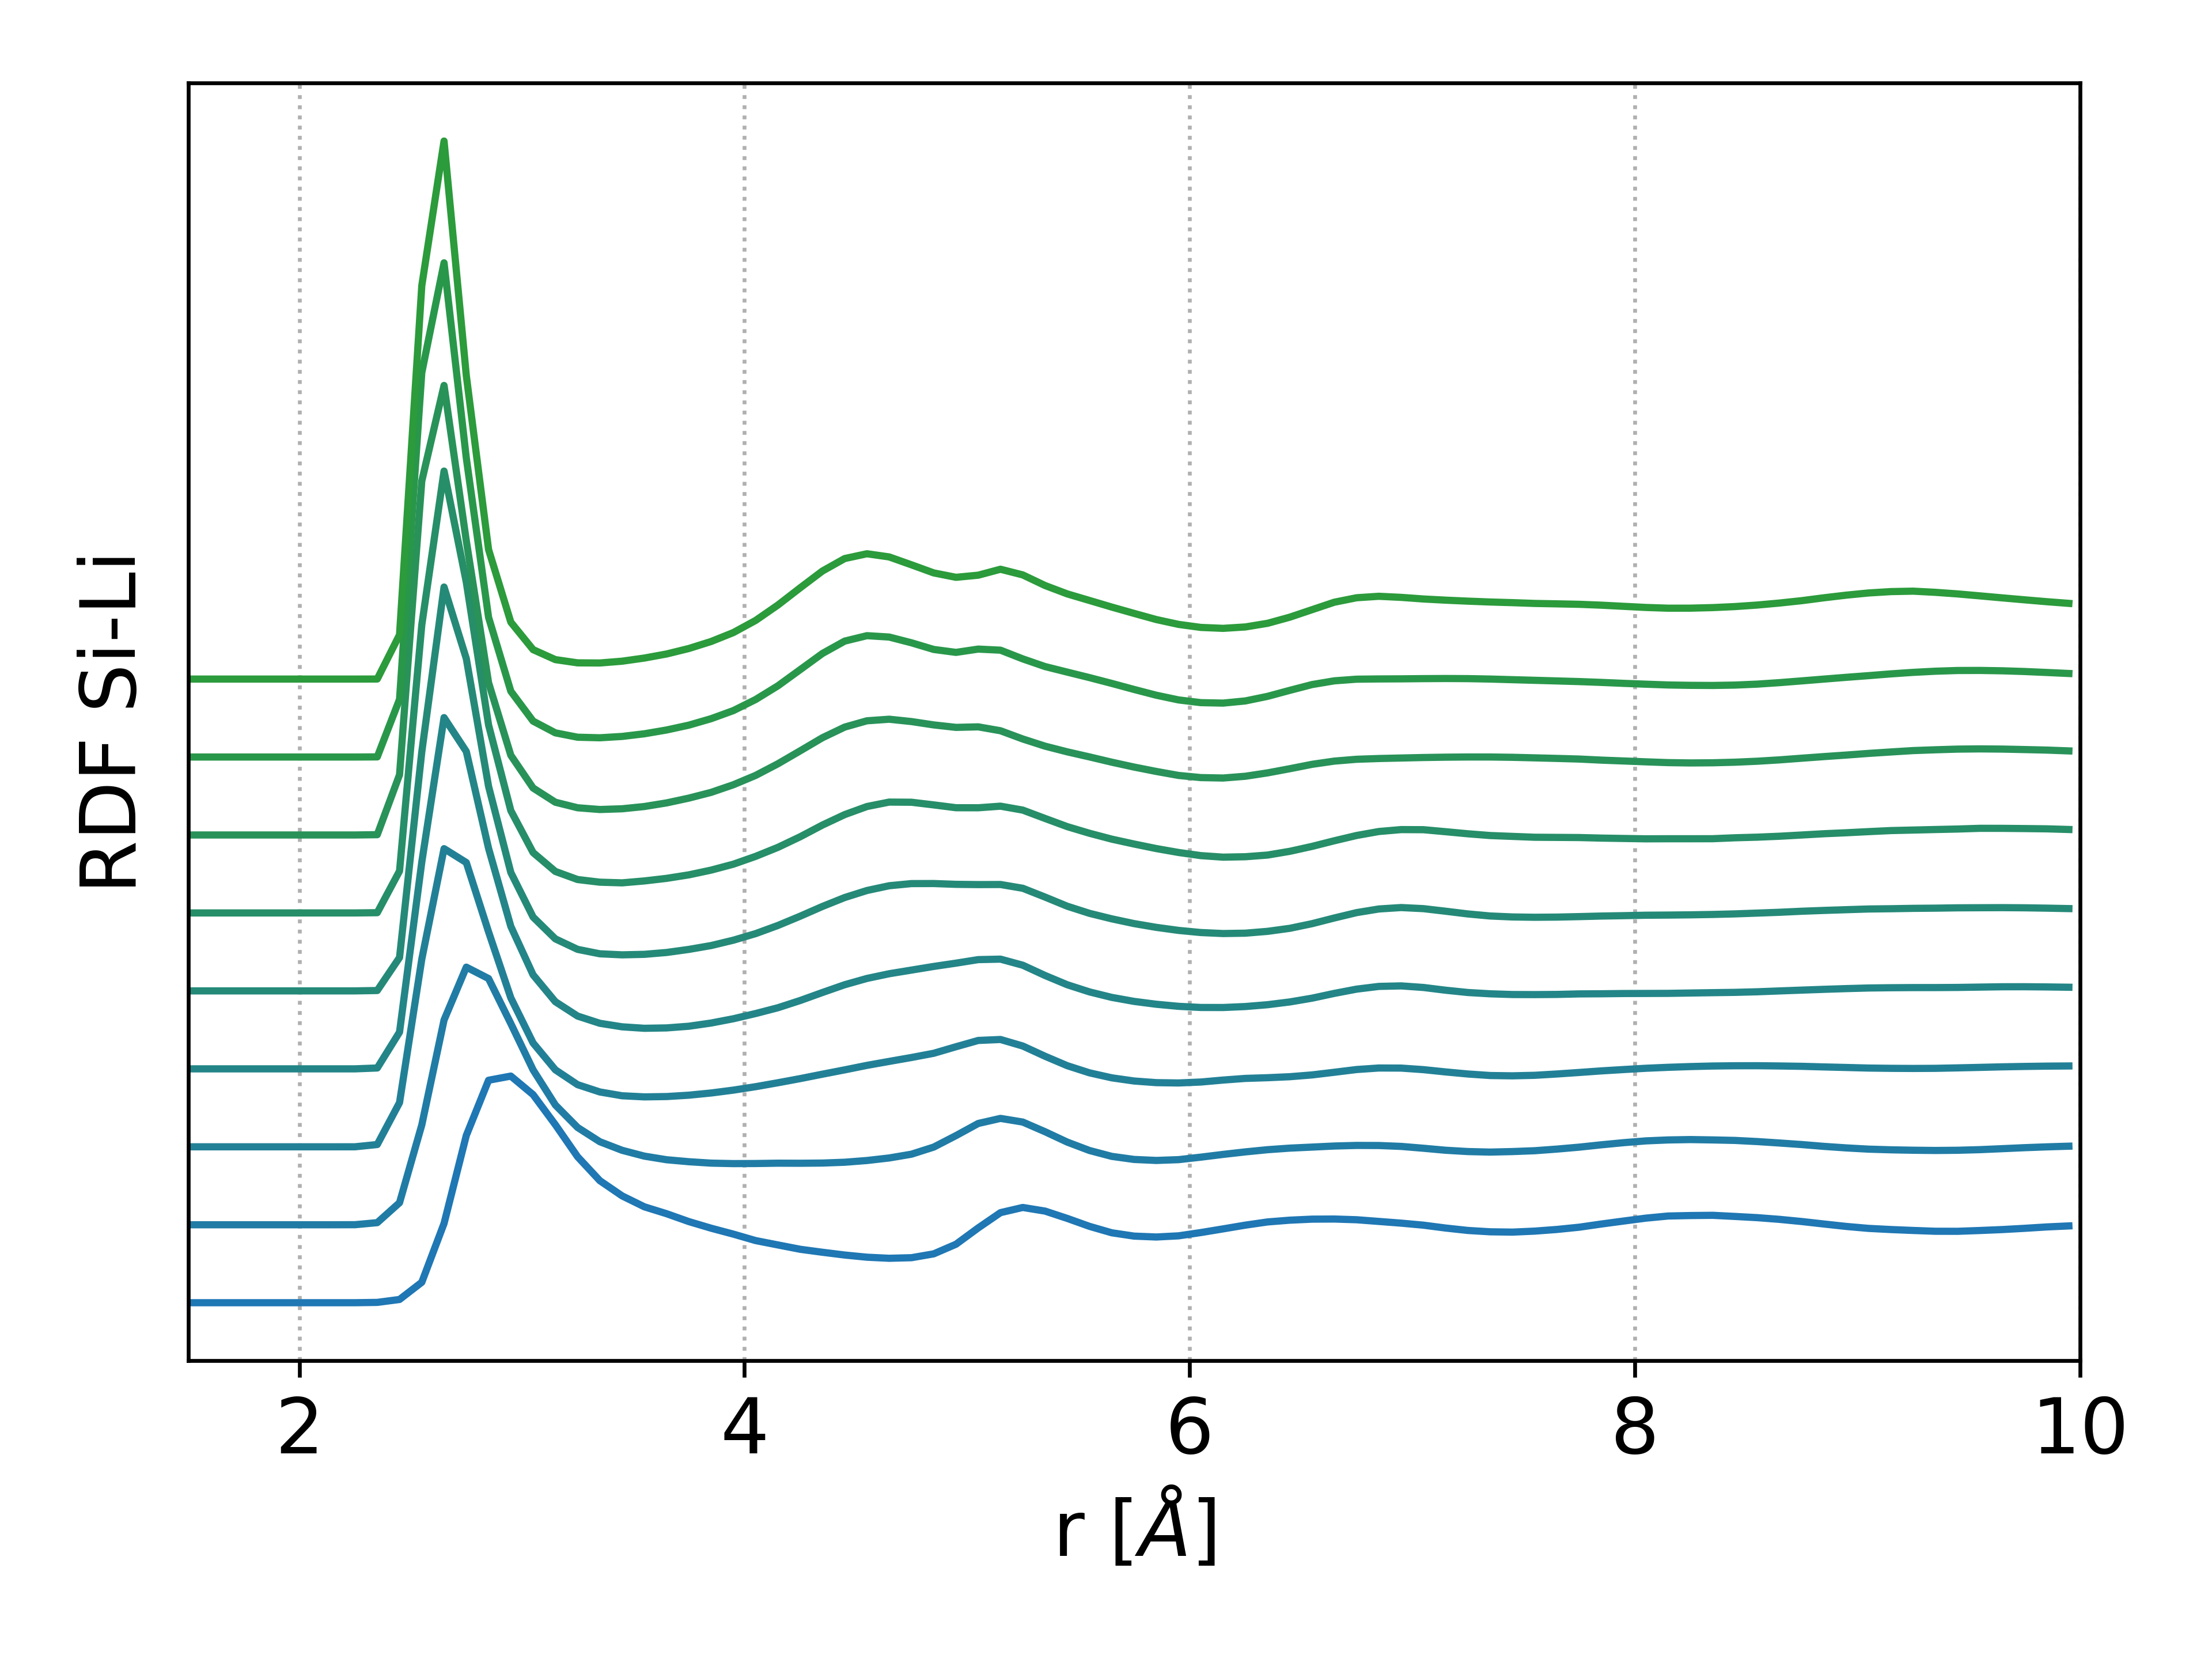
\includegraphics[width=0.8\textwidth]{caracterizacion/rdf-SiLi.png}
    \caption{Distribución radial de a pares para Si-Li de las estructuras 
    minimizadas. Cada curva se corresponde con un valor de concentración 
    distinto.}
    \label{fig:rdf-SiLi}
\end{figure}
Para el primer pico de la RDF$_{Si-Li}$ se ve el comportamiento contrario, el 
centro del mismo se desplaza a distancias menores a medida que la concentración
de litio aumenta. Esto es acompañado con un aumento de la altura del pico y una
disminución de su ancho. Para el segundo pico también se observa un desplazamiento
del mismo hacia distancias menores, pero por encima de $x = 1.71$ el pico se
divide en dos picos con distintas alturas dependiendo de la concentración. Esto
es analizado con mayor detalle en la sección \ref{s:intercionexion}.

\subsection{Número de coordinación}

De la misma manera que se definió la distribuciones radiales de a pares parciales,
se pueden obtener los números de coordinación a un dado tipo de átomos. CN$_{ij}$
se corresponde con la cantidad de átomos vecinos de tipo $j$ para un átomo central 
de tipo $i$ hasta una cierta distancia de corte. Para la elección de dicho valor 
se considera hasta el primer pico de la $g_{ij}(r)$ correspondiente. Debido a que 
en los materiales amorfos la primera y la segunda esfera de coordinación pueden 
llegar a estar superpuestas, el límite superior de integración no está definido 
unívocamente para todas las concentraciones consideradas ~\cite{lamparter1995}.
Para el número de coordinación promedio para átomos de Si vecinos de otros átomos 
de Si se calculó contando el número de dichos vecinos utilizando un radio de 
corte de 3 \AA. Lo mismo se realizó para Li-Li definiendo un radio de corte de 
4 \AA. Para el caso de Si-Li se utilizó el criterio de considerar como radio de 
corte el valor $r$ para el cual la $g(r)$ presenta un mínimo entre los dos picos
a primeros y segundo vecinos. Los resultados se muestran en la figura 
\ref{fig:cn1}.
\begin{figure}[th]
    \centering
    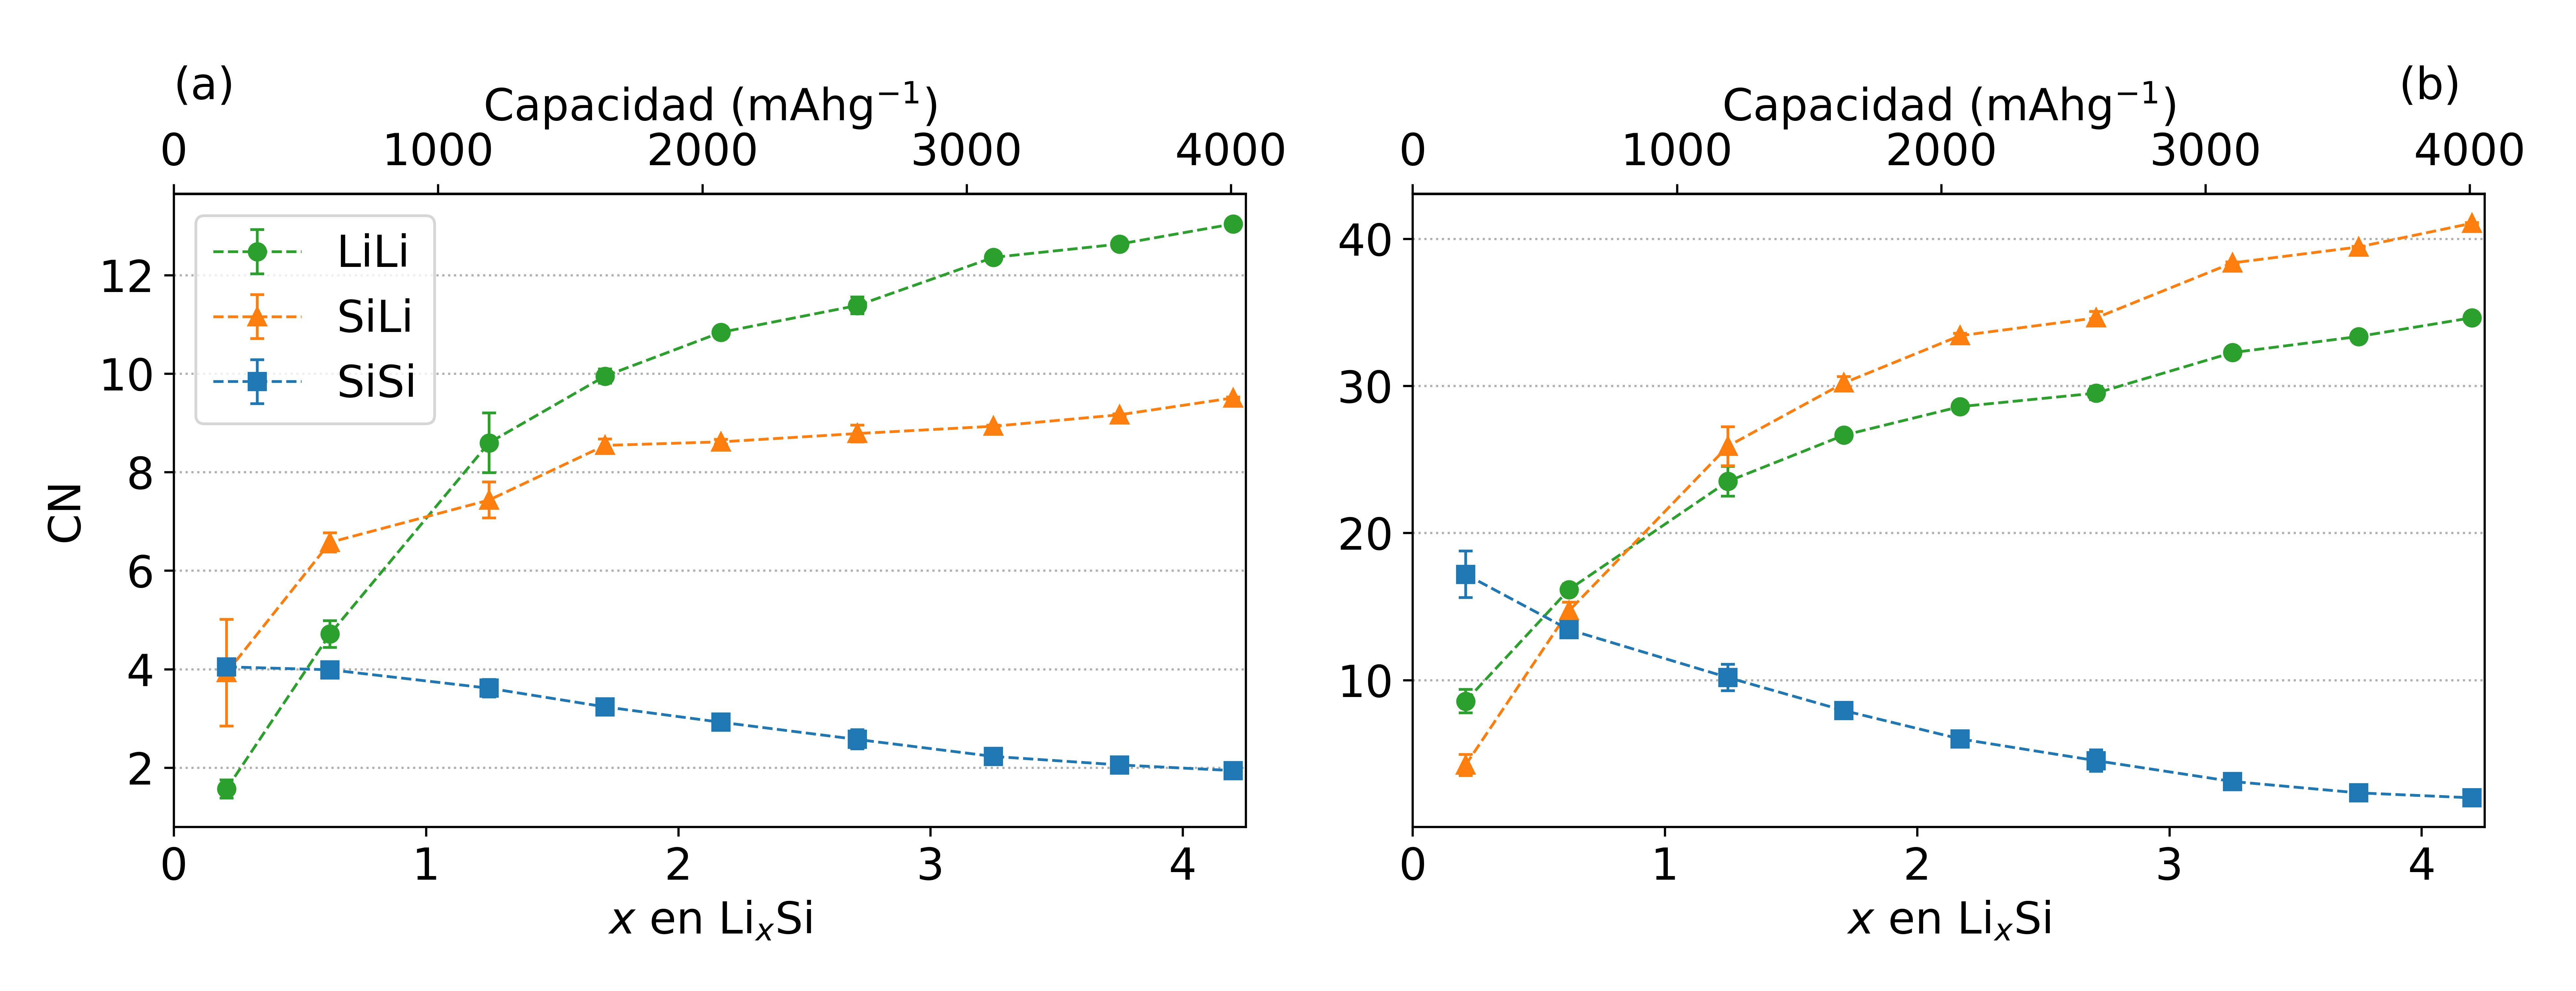
\includegraphics[width=0.8\textwidth]{caracterizacion/cn.png}
    \caption{Promedio del primer número de coordinación en función de la 
    concentración de litio para Li-Li, Si-Si y Si-Li. Como radio de corte se 
    utilizó la distancia posterior al primer pico de la RDF correspondiente. En 
    los casos que no se aprecia la barra de error, es porque la misma es menor 
    que el tamaño de los puntos.}
    \label{fig:cn1}
\end{figure}

Para el caso del CN$_{Si-Si}$, se tiene que esta cantidad decrece de 4 a 2, a 
medida que la concentración de Li aumenta. Esto indica que a valores pequeños de 
$x$ la estructura de Si mantiene sus conexiones tetraédricas, mientras que para
valores grandes de $x$ el Si tiende a formar cadenas periódicas unidimensionales.
En la red de silicio amorfa, analizada con más detalle en la sección 
\ref{s:clusters}, una estructura 3-periódica se presenta para valores bajos de 
$x$, donde el CN se encuentra alrededor de 4. Luego, una estructura 1-periódica se
alcanza para valores grandes de $x$, donde los enlaces Si-Si tienden a formar 
cadenas, que pueden verse para $x = 3.75$ donde se tiene $CN = 2.05$, por ejemplo.
El CN de Si-Li y Li-Li presenta valores pequeños para concentraciones 
bajas y aumenta monótonamente hasta alcanzar valores de 10 y 12, respectivamente, 
que se asemejan al valor de una estructura de empaquetamiento compacto.

\begin{figure}[th]
    \centering
    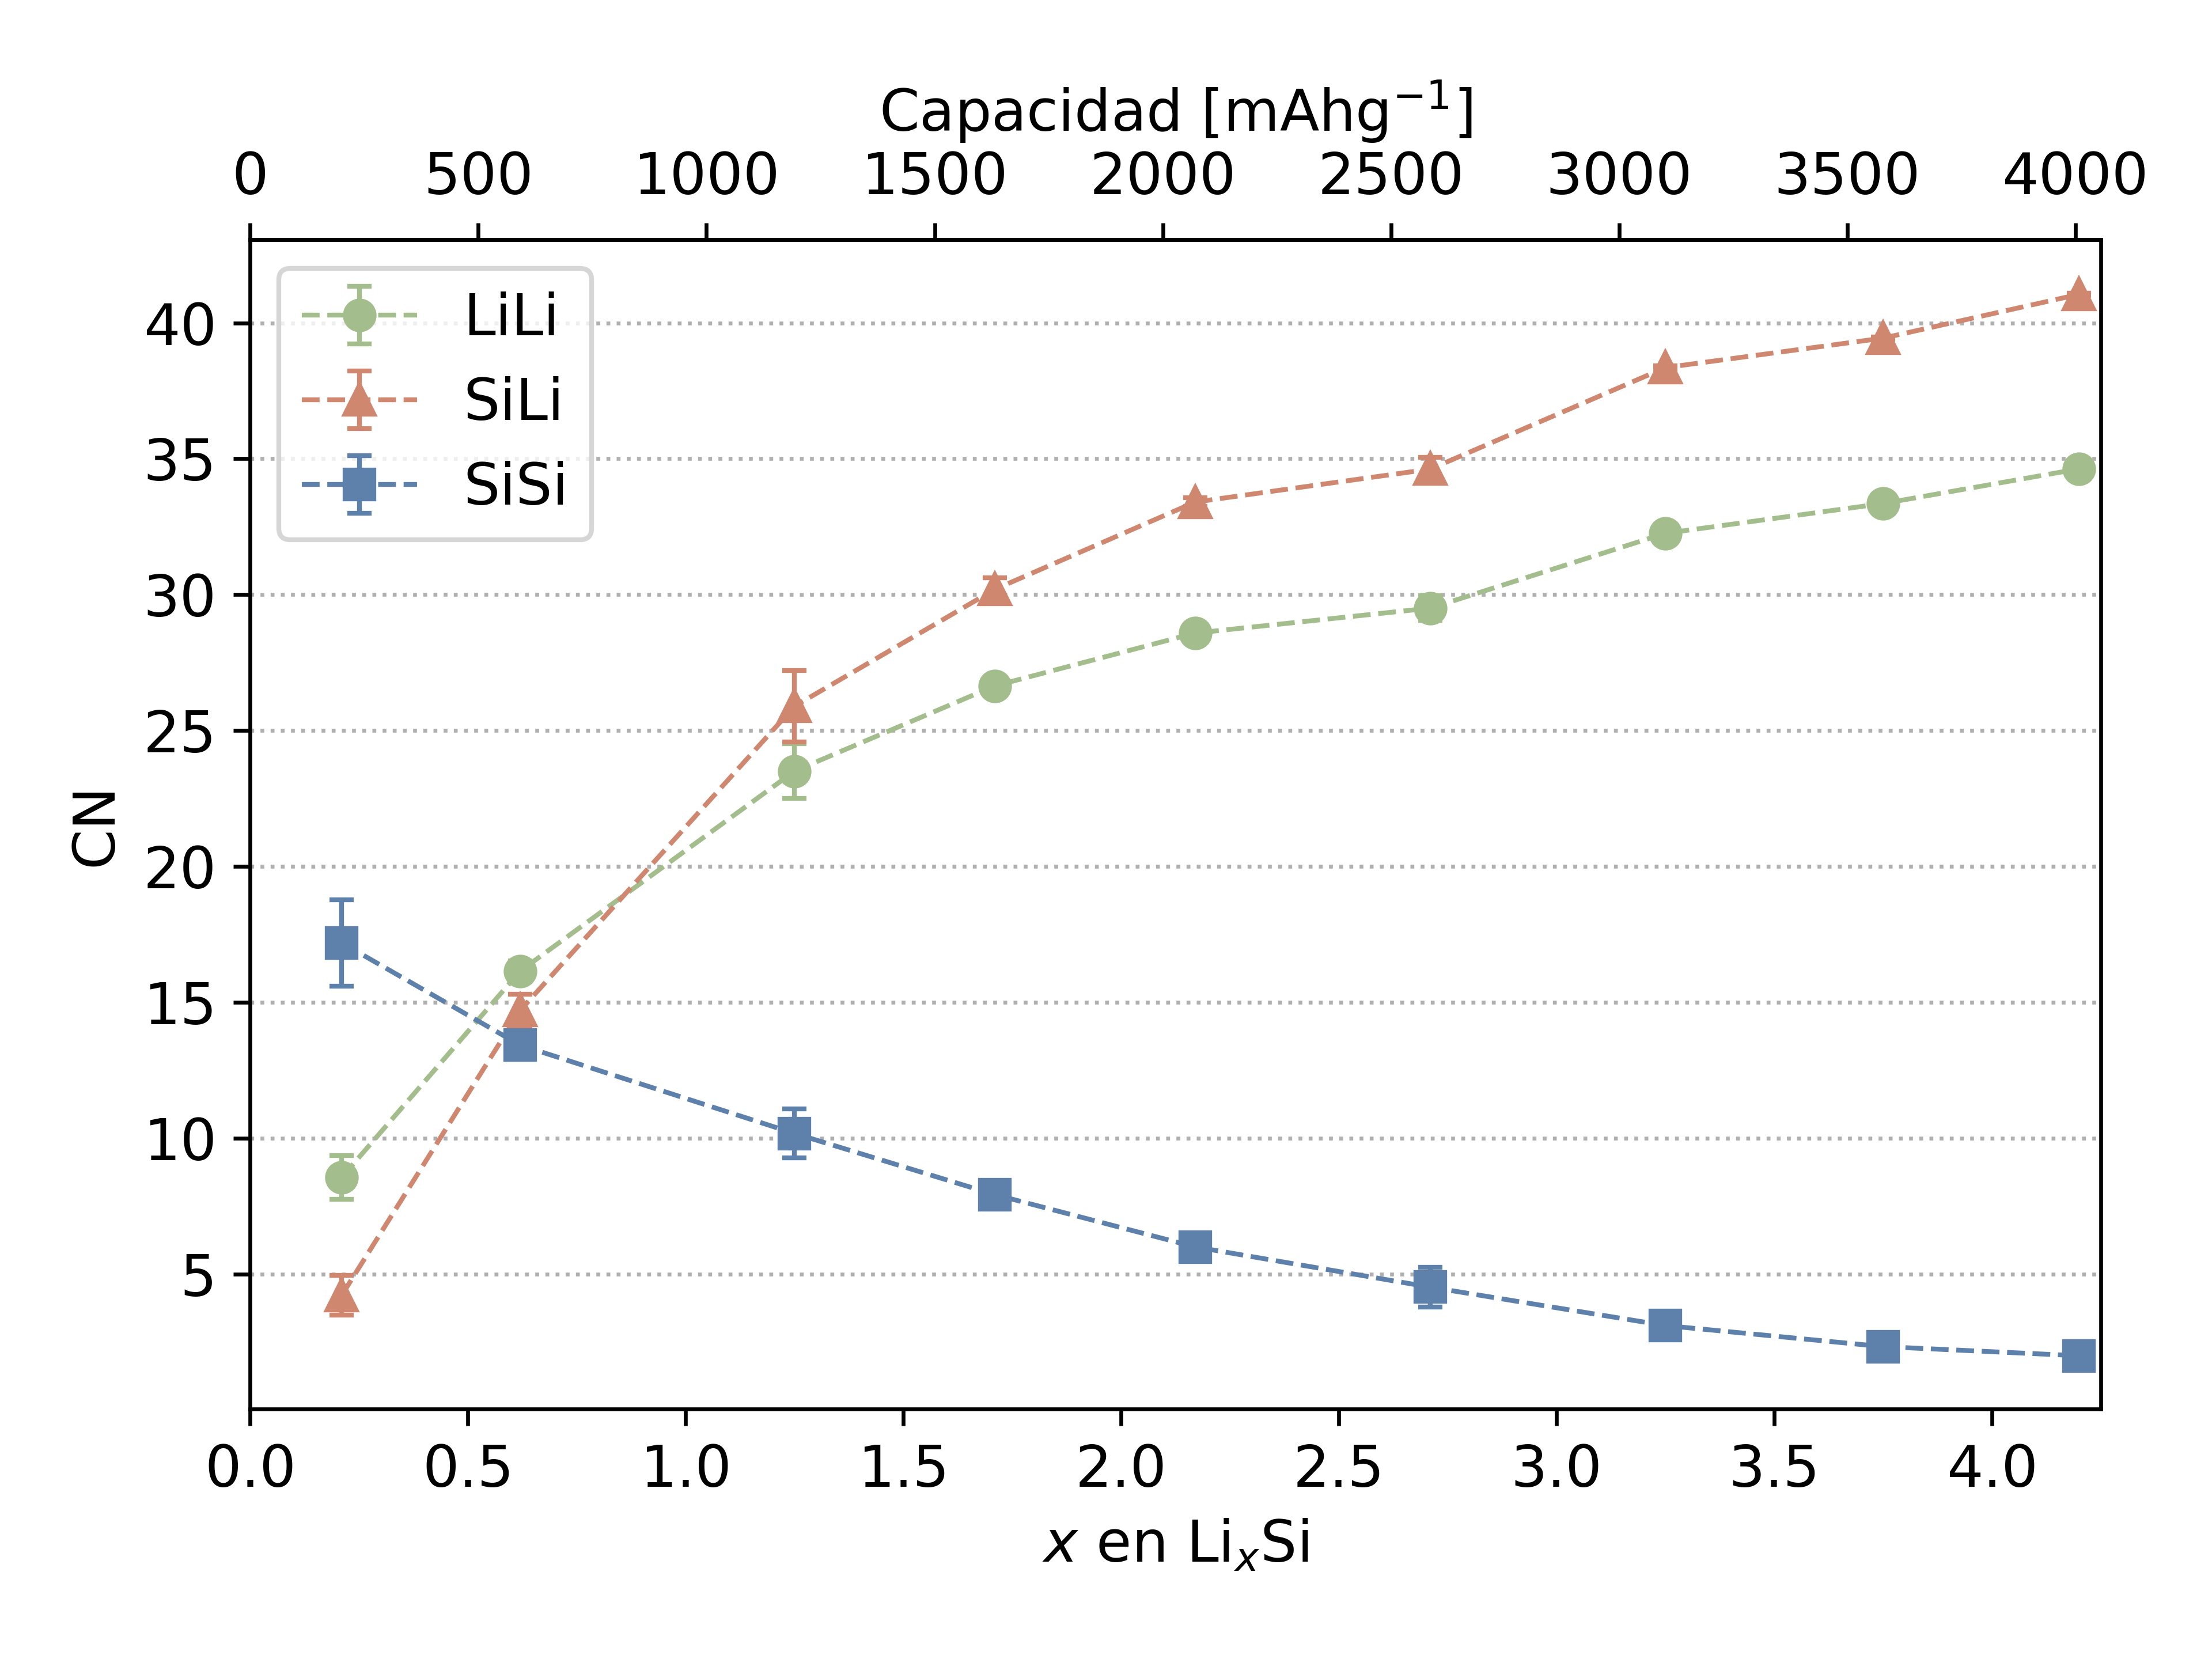
\includegraphics[width=0.8\textwidth]{caracterizacion/cn2.png}
    \caption{Promedio del segundo número de coordinación en función de la 
    concentración de litio para Li-Li, Si-Si y Si-Li. Para la elección de los 
    radios de corte que definen el cascarón en el cual se cuentan los vecinos,
    se consideró el segundo pico de la RDF correspondiente. En los casos que no 
    se aprecia la barra de error, es porque la misma es menor que el tamaño de 
    los puntos.}
    \label{fig:cn2}
\end{figure}
Los resultados para el segundo número de coordinación se presentan en la figura 
\ref{fig:cn2}. Estos resultados se obtuvieron considerando un cascarón con un 
radio de corte interno y otro externo, elegidos de manera tal que incluyan el 
segundo pico de la RDF. La elección de dichos valores varió dependiendo del tipo
de átomos que se consideraron. En todos ellos se tomó como radio de corte interno 
el radio de corte del primero número de coordinación. Luego, para el radio de 
corte externo se utilizaron valores de 5.0 \AA\ para Si-Si y 6.0 \AA\ para Li-Li
y Si-Li.

Para los valores de CN$_{Si-Si}$ se observa un aumento para concentraciones bajas
de Li si se lo compara con el CN de primeros vecinos. Para valores mayores de $x$,
se puede ver como el valor de CN también tiende a 2, lo cual es coherente con la
formación de cadenas que se notó previamente. La tendencia cualitativa del segundo
CN para Li-Li y Si-Li es la misma a la observada en el primer CN, sólo que ahora
empieza en un valor cercano a 5 y tiende a 35 y 40, respectivamente. Este valor 
es mucho mayor que el que se tiene para los segundos vecinos en una estructura 
de empaquetamiento compacto, que es 6 para la estructura cristalina FCC. Incluso 
es mayor a la suma del segundo (6) y del tercer vecino (24) esperado para la red 
FCC.

\subsection{Formación de clusters}\label{s:clusters}

Analizando la formación de clusters por medio del algoritmo DBSCAN 
~\cite{ester1996}, en el cual puede definirse un radio de corte para el cual se 
deja de considerar que los átomos están enlazados entre sí (es decir, formando 
clusters), se encuentra que las estructuras amorfas de silicio no pueden ser 
clasificadas en diferentes tipos de clusters, las mismas reflejan más bien 
una red amorfa. Esto viene de interpretar los gráficos que se presentan en la 
figura \ref{fig:clusters}. 

En particular, en la figura \ref{fig:clusters-isolated} se define el porcentaje 
de átomos de Si que están a una distancia mayor que $r_{cut}$ de otros átomos de 
Si, cuando el radio de corte es mayor que la distancia a la cual termina el 
primer pico de la RDF$_{Si-Si}$, no se tienen átomos de Si que cumplan esta 
propiedad, es decir, no hay átomos de Si que se encuentren aislados en el sistema, 
incluso a concentraciones altas de Li. Esto refleja que el a-Si se comporta como 
una red en la cual todos los átomos de silicio están interconectados entre sí, 
que también se puede deducir de la figura \ref{fig:clusters-nclusters} en la cual 
se tiene que cuando el radio de corte es menor al primer pico de la RDF$_{Si-Si}$ 
el número de clusters es igual al número de átomos de Si, pero que cuando este 
radio es más grande que la distancia a la cual termina el primer pico, hay un 
solo cluster.

\begin{figure}[h]
    \centering
    \begin{subfigure}{.475\textwidth}
        \centering
        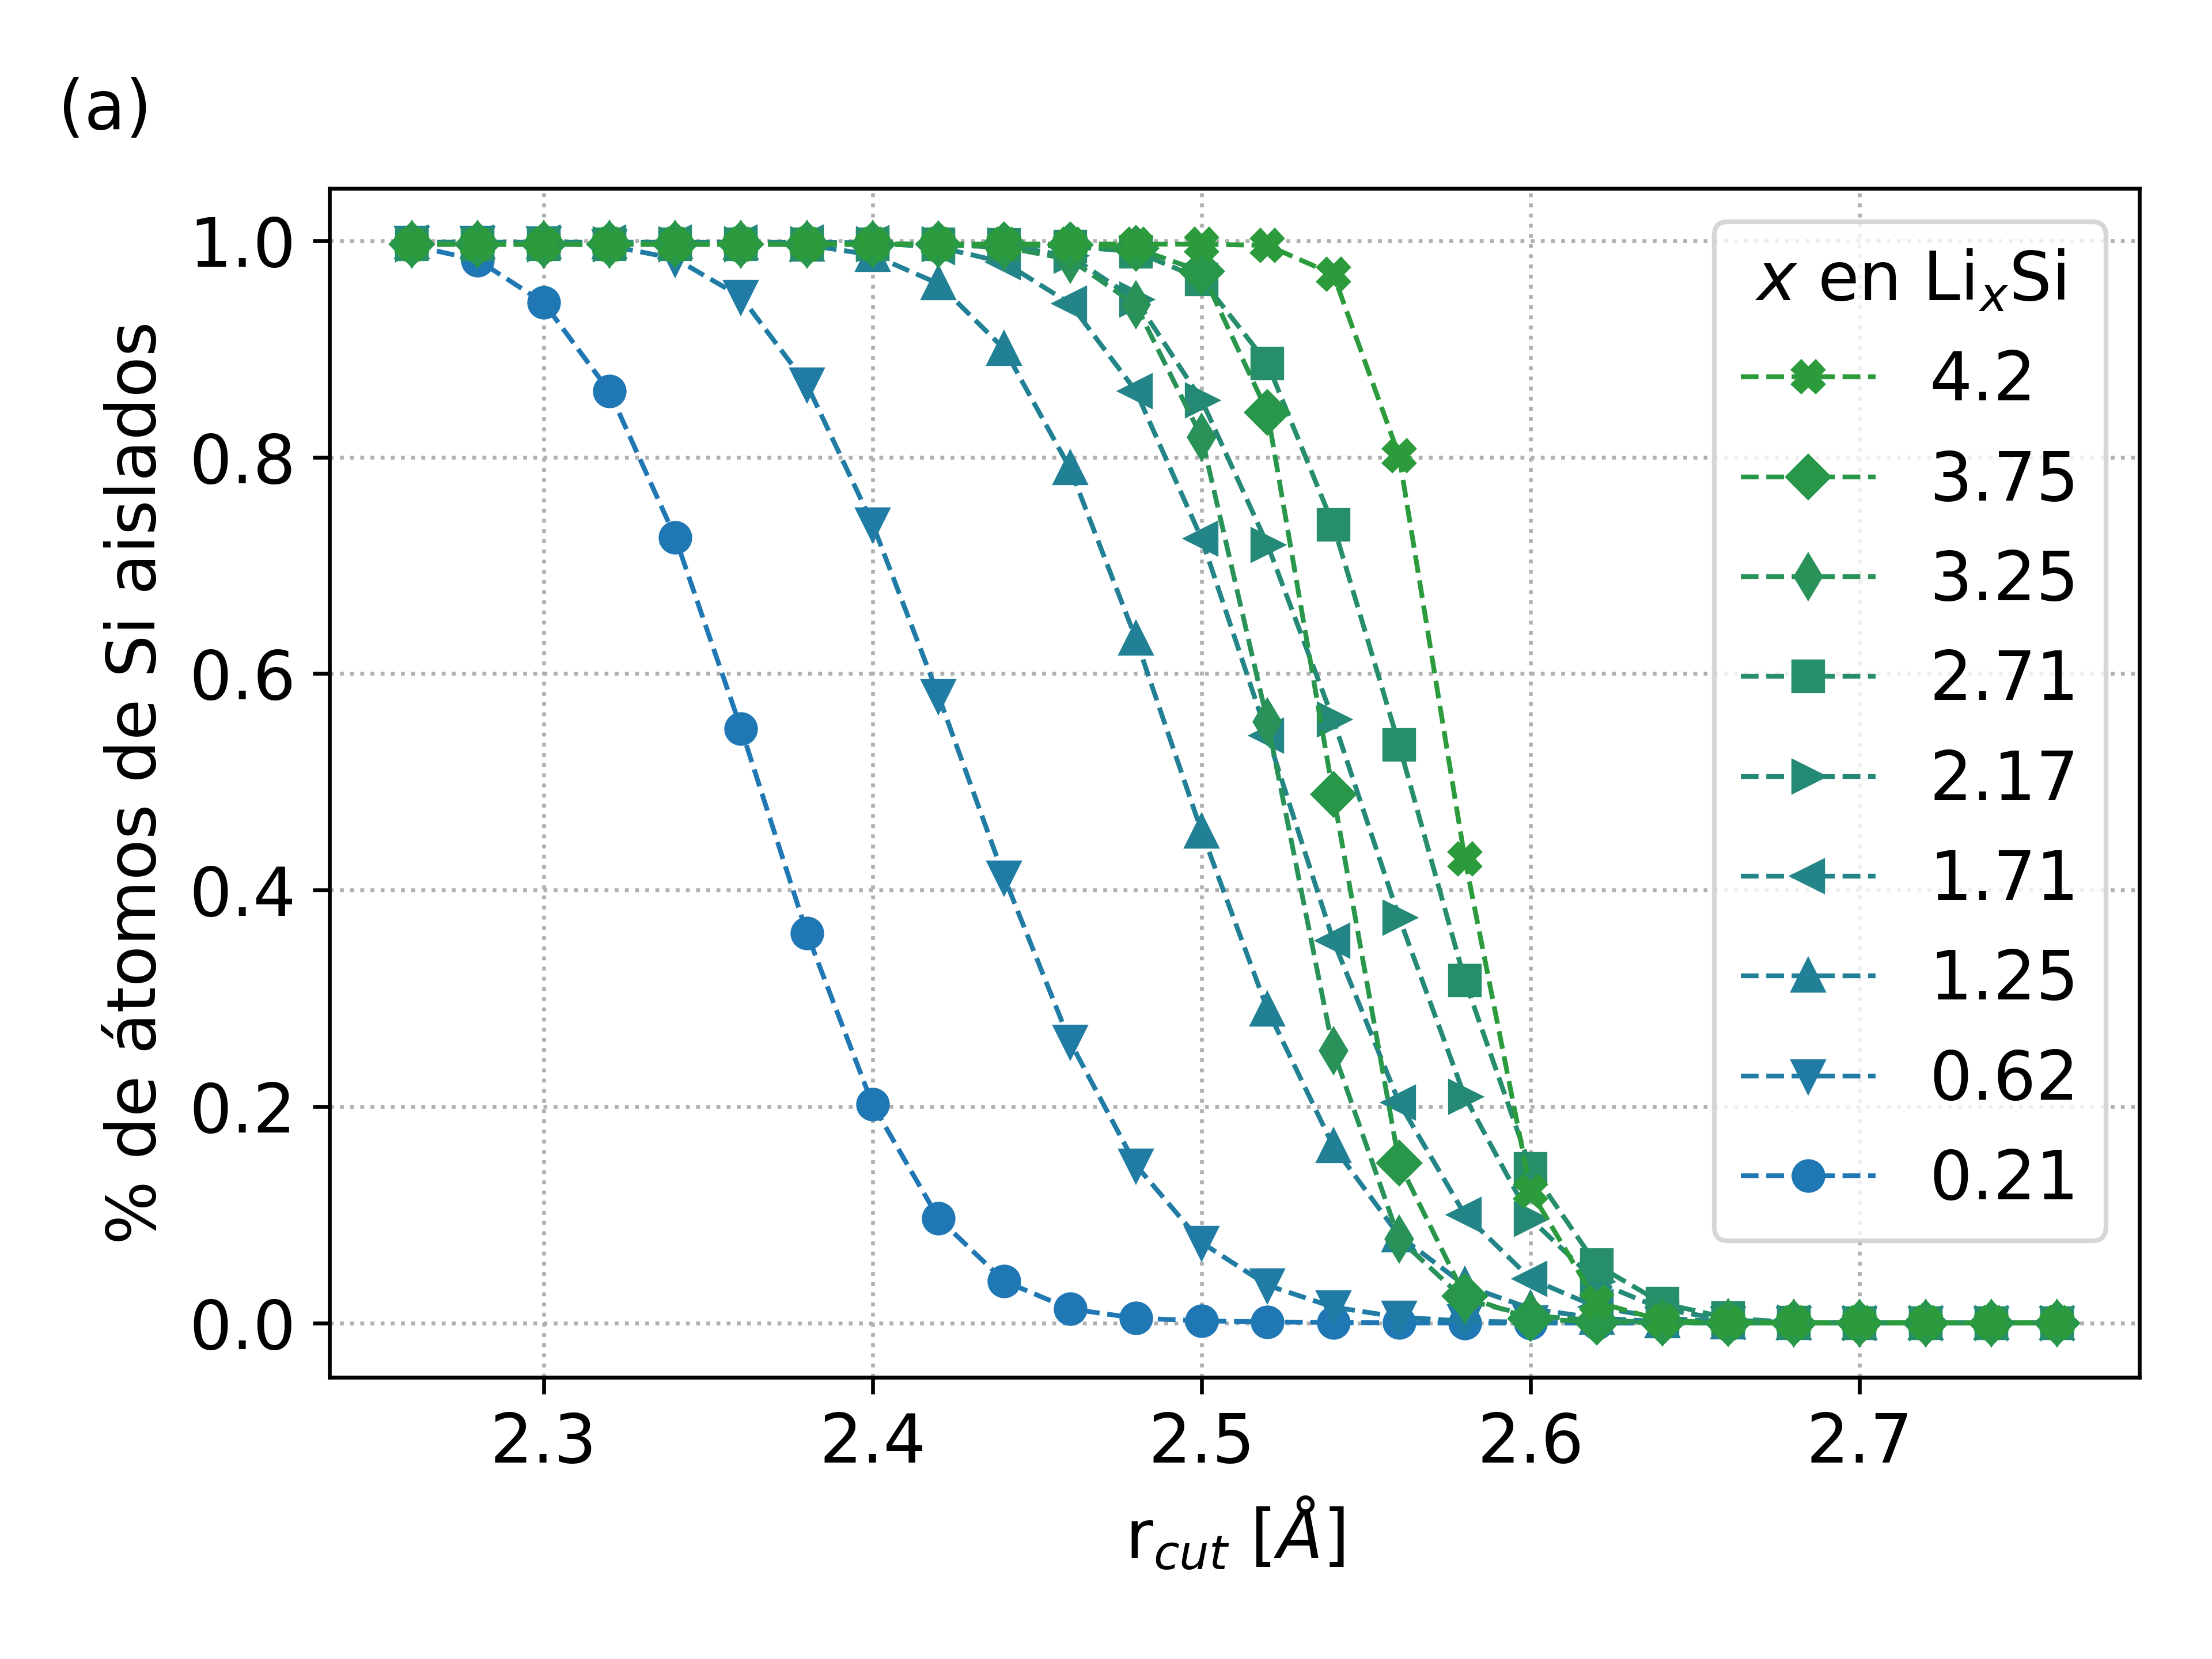
\includegraphics[width=\textwidth]{caracterizacion/cluster-isolated.png}
        \caption{Porcentaje de átomos de Si aislados en función de la elección del
        radio de corte.}
        \label{fig:clusters-isolated}
    \end{subfigure}
    \hfill
    \begin{subfigure}{.475\textwidth}
        \centering
        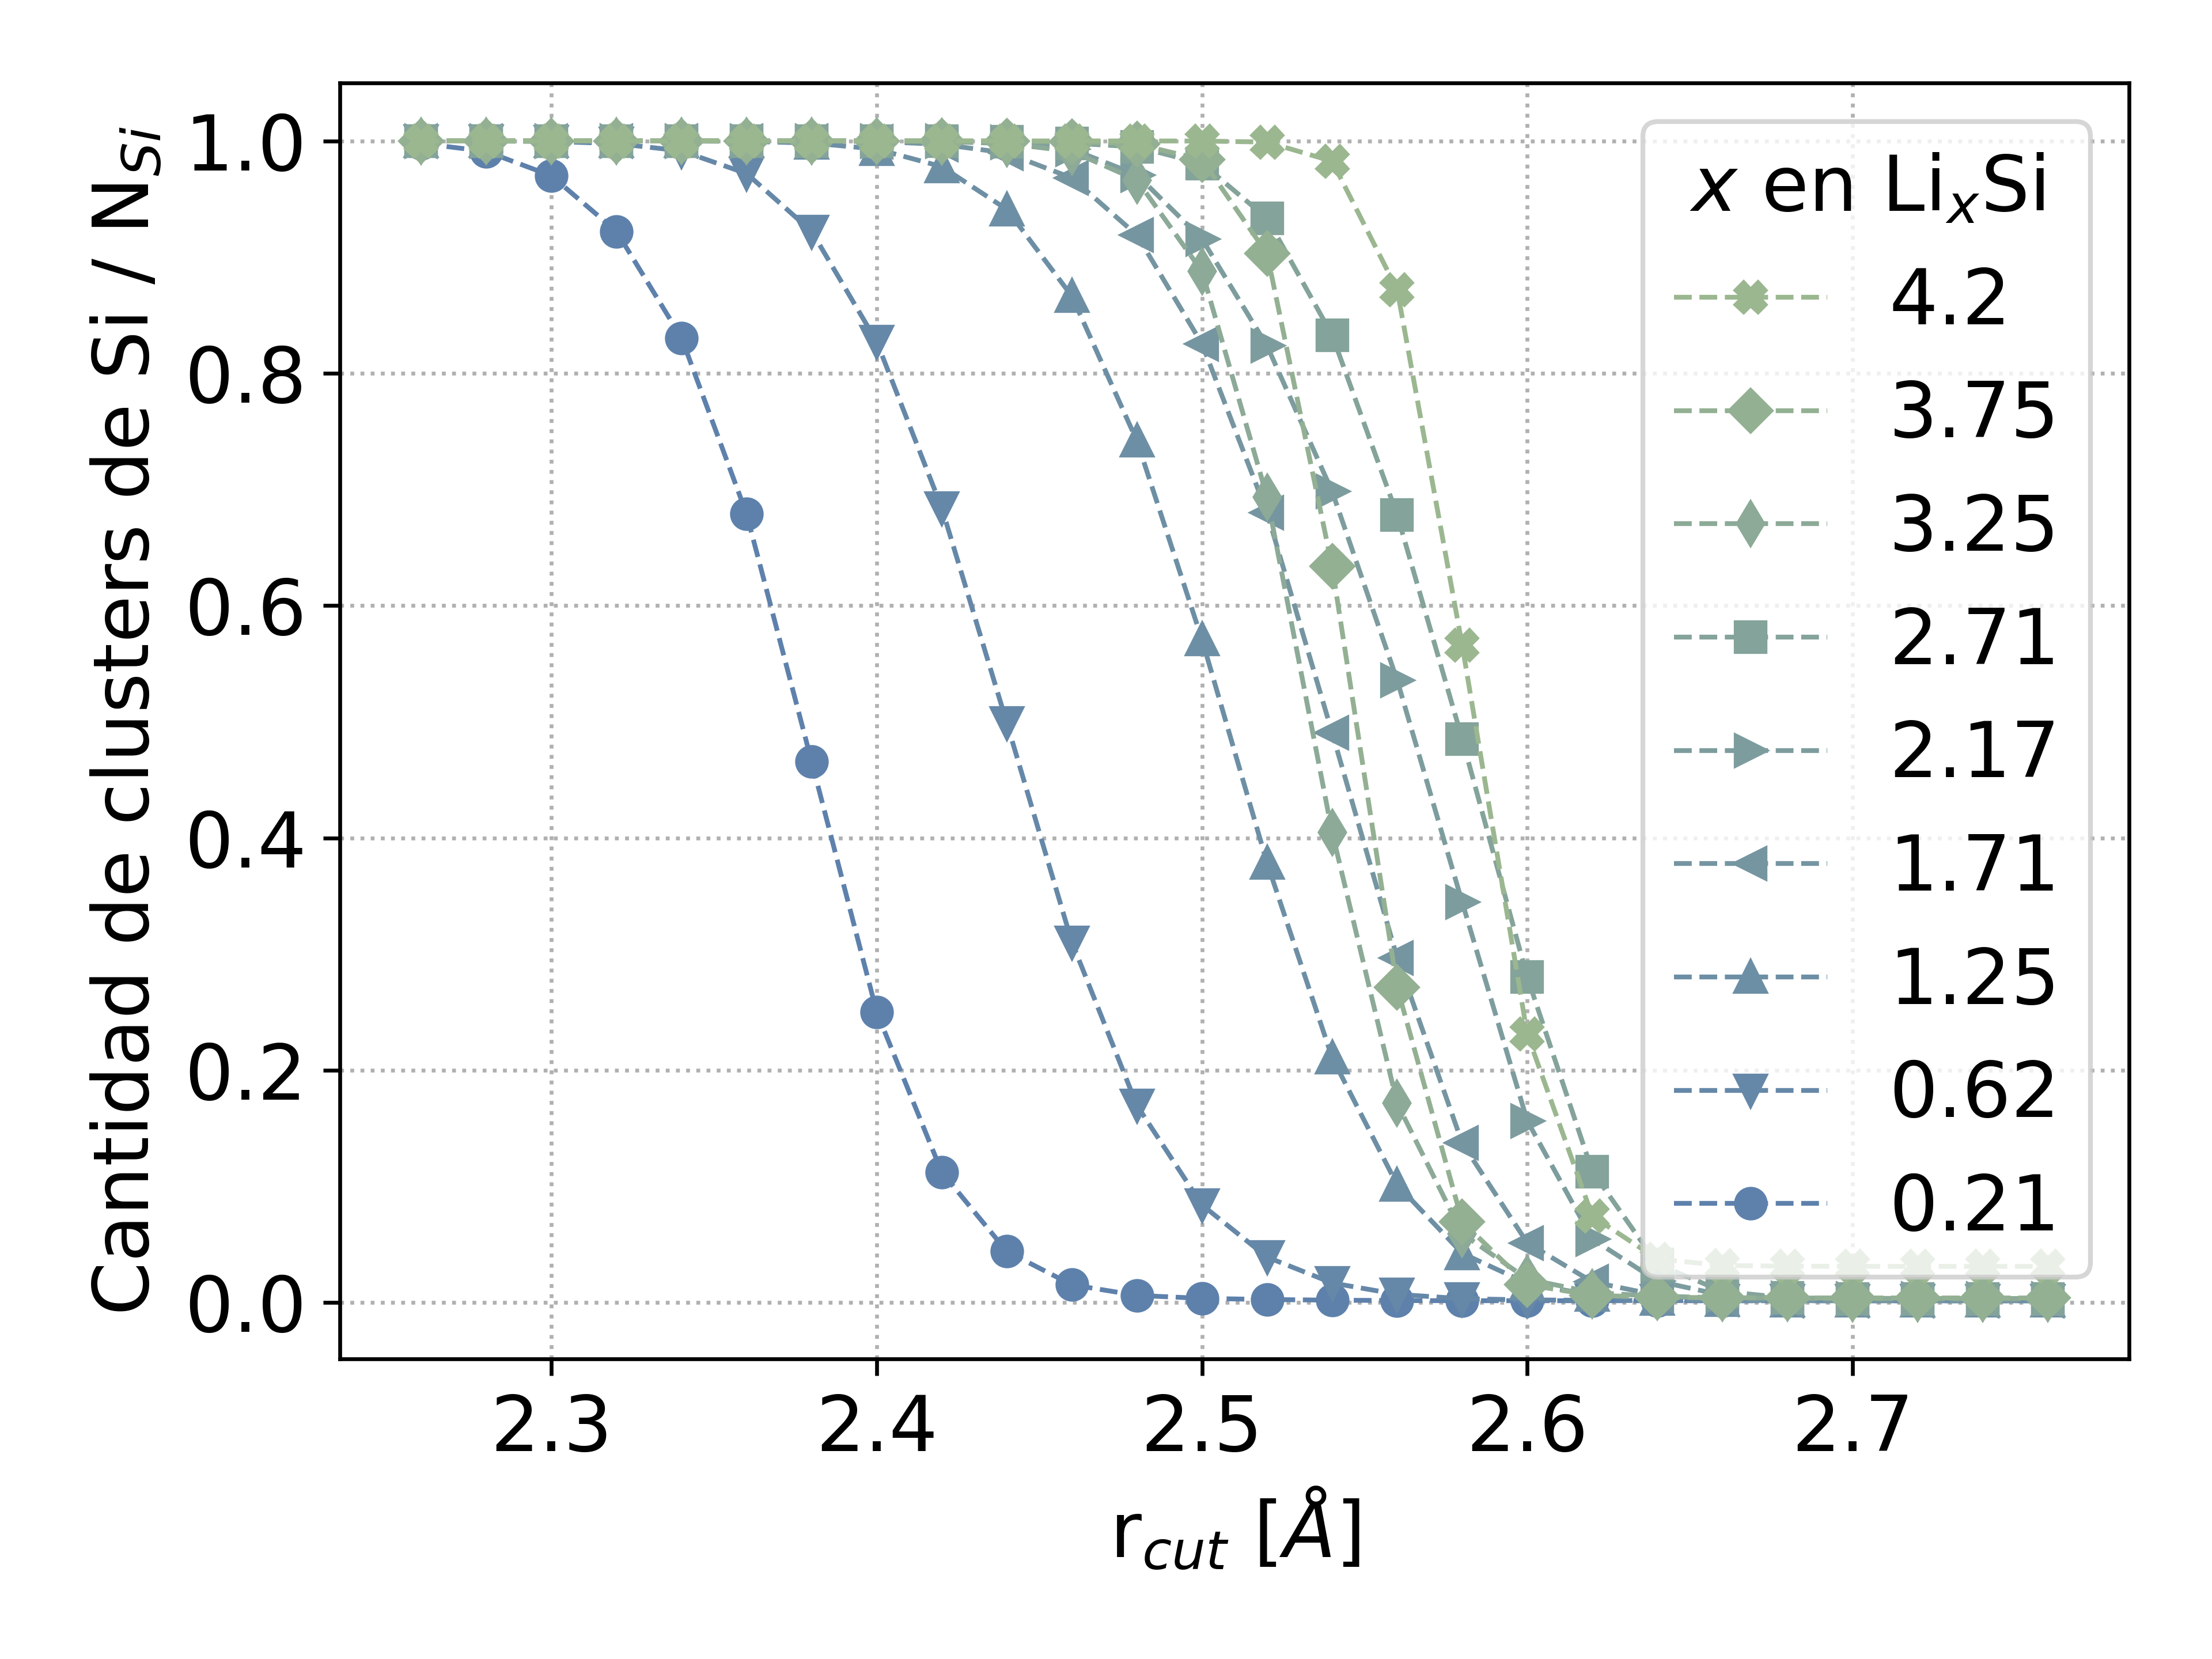
\includegraphics[width=\textwidth]{caracterizacion/cluster-nclusters.png}
        \caption{Número de clusters de Si sobre el número total de átomos de Si.}
        \label{fig:clusters-nclusters}
    \end{subfigure}
    \caption{Formación de clusters indicando una red amorfa de silicio.}
    \label{fig:clusters}
\end{figure}

\subsection{Interconexión de clusters}\label{s:intercionexion}

Para determinar que es lo que causa la división en el segundo pico de la 
RDF$_{Si-Li}$ se realizó un análisis similar al reportado por Ding \textit{et al.}
~\cite{ding2015}. Estos autores analizaron la correlación en la distancia de a
pares de los segundos vecinos más cercanos en términos de las conexiones entre
clusters, definiendo un poliedro de coordinación alrededor del átomo central 
considerado para la RDF y sus segundos vecinos. El número de átomos compartidos
entre estos dos poliedros de coordinación enlazados fueron utilizados para 
establecer categorías y analizar sus contribuciones a la RDF. Estas categorías
dependen del hecho de que los poliedros comparten un vértice (1 átomo), una 
arista (2 átomos), una cara de los poliedros (3 átomos) o cuadriláteros 
distorsionados o tetraedros aplastados (4 átomos). De una forma similar a este 
trabajo, se deconvolucionó el segundo pico de la RDF calculando la RDF parcial 
de distintas categorías, donde cada categoría se define por el número de átomos de
Li que interconectan un átomo de Si con su segundo vecino de Li. El comportamiento
detallado se presenta en la figura \ref{fig:interconexiones}. Puede afirmarse a 
grandes rasgos que para concentraciones bajas de Li en las aleaciones, hay una 
predominancia de segundos vecinos de Li que tienen una o ninguna interconexión 
con los vecinos de Li de la primera esfera de coordinación Si-Li. Para $x > 1.0$
la contribución del segundo vecino de Li interconectado con dos o más átomos de 
Li de la primera esfera de coordinación Si-Li comienza a ser predominante y la
contribución de los átomos de Li sin conectarse empieza a decaer. Para $x > 3.0$,
la contribución del primer pico del segundo vecino de Li interconectado dos o
tres veces se vuelve relevante mientras que aparecen contribuciones de cuatro o
más interconexiones.
\begin{figure}[th]
    \centering
    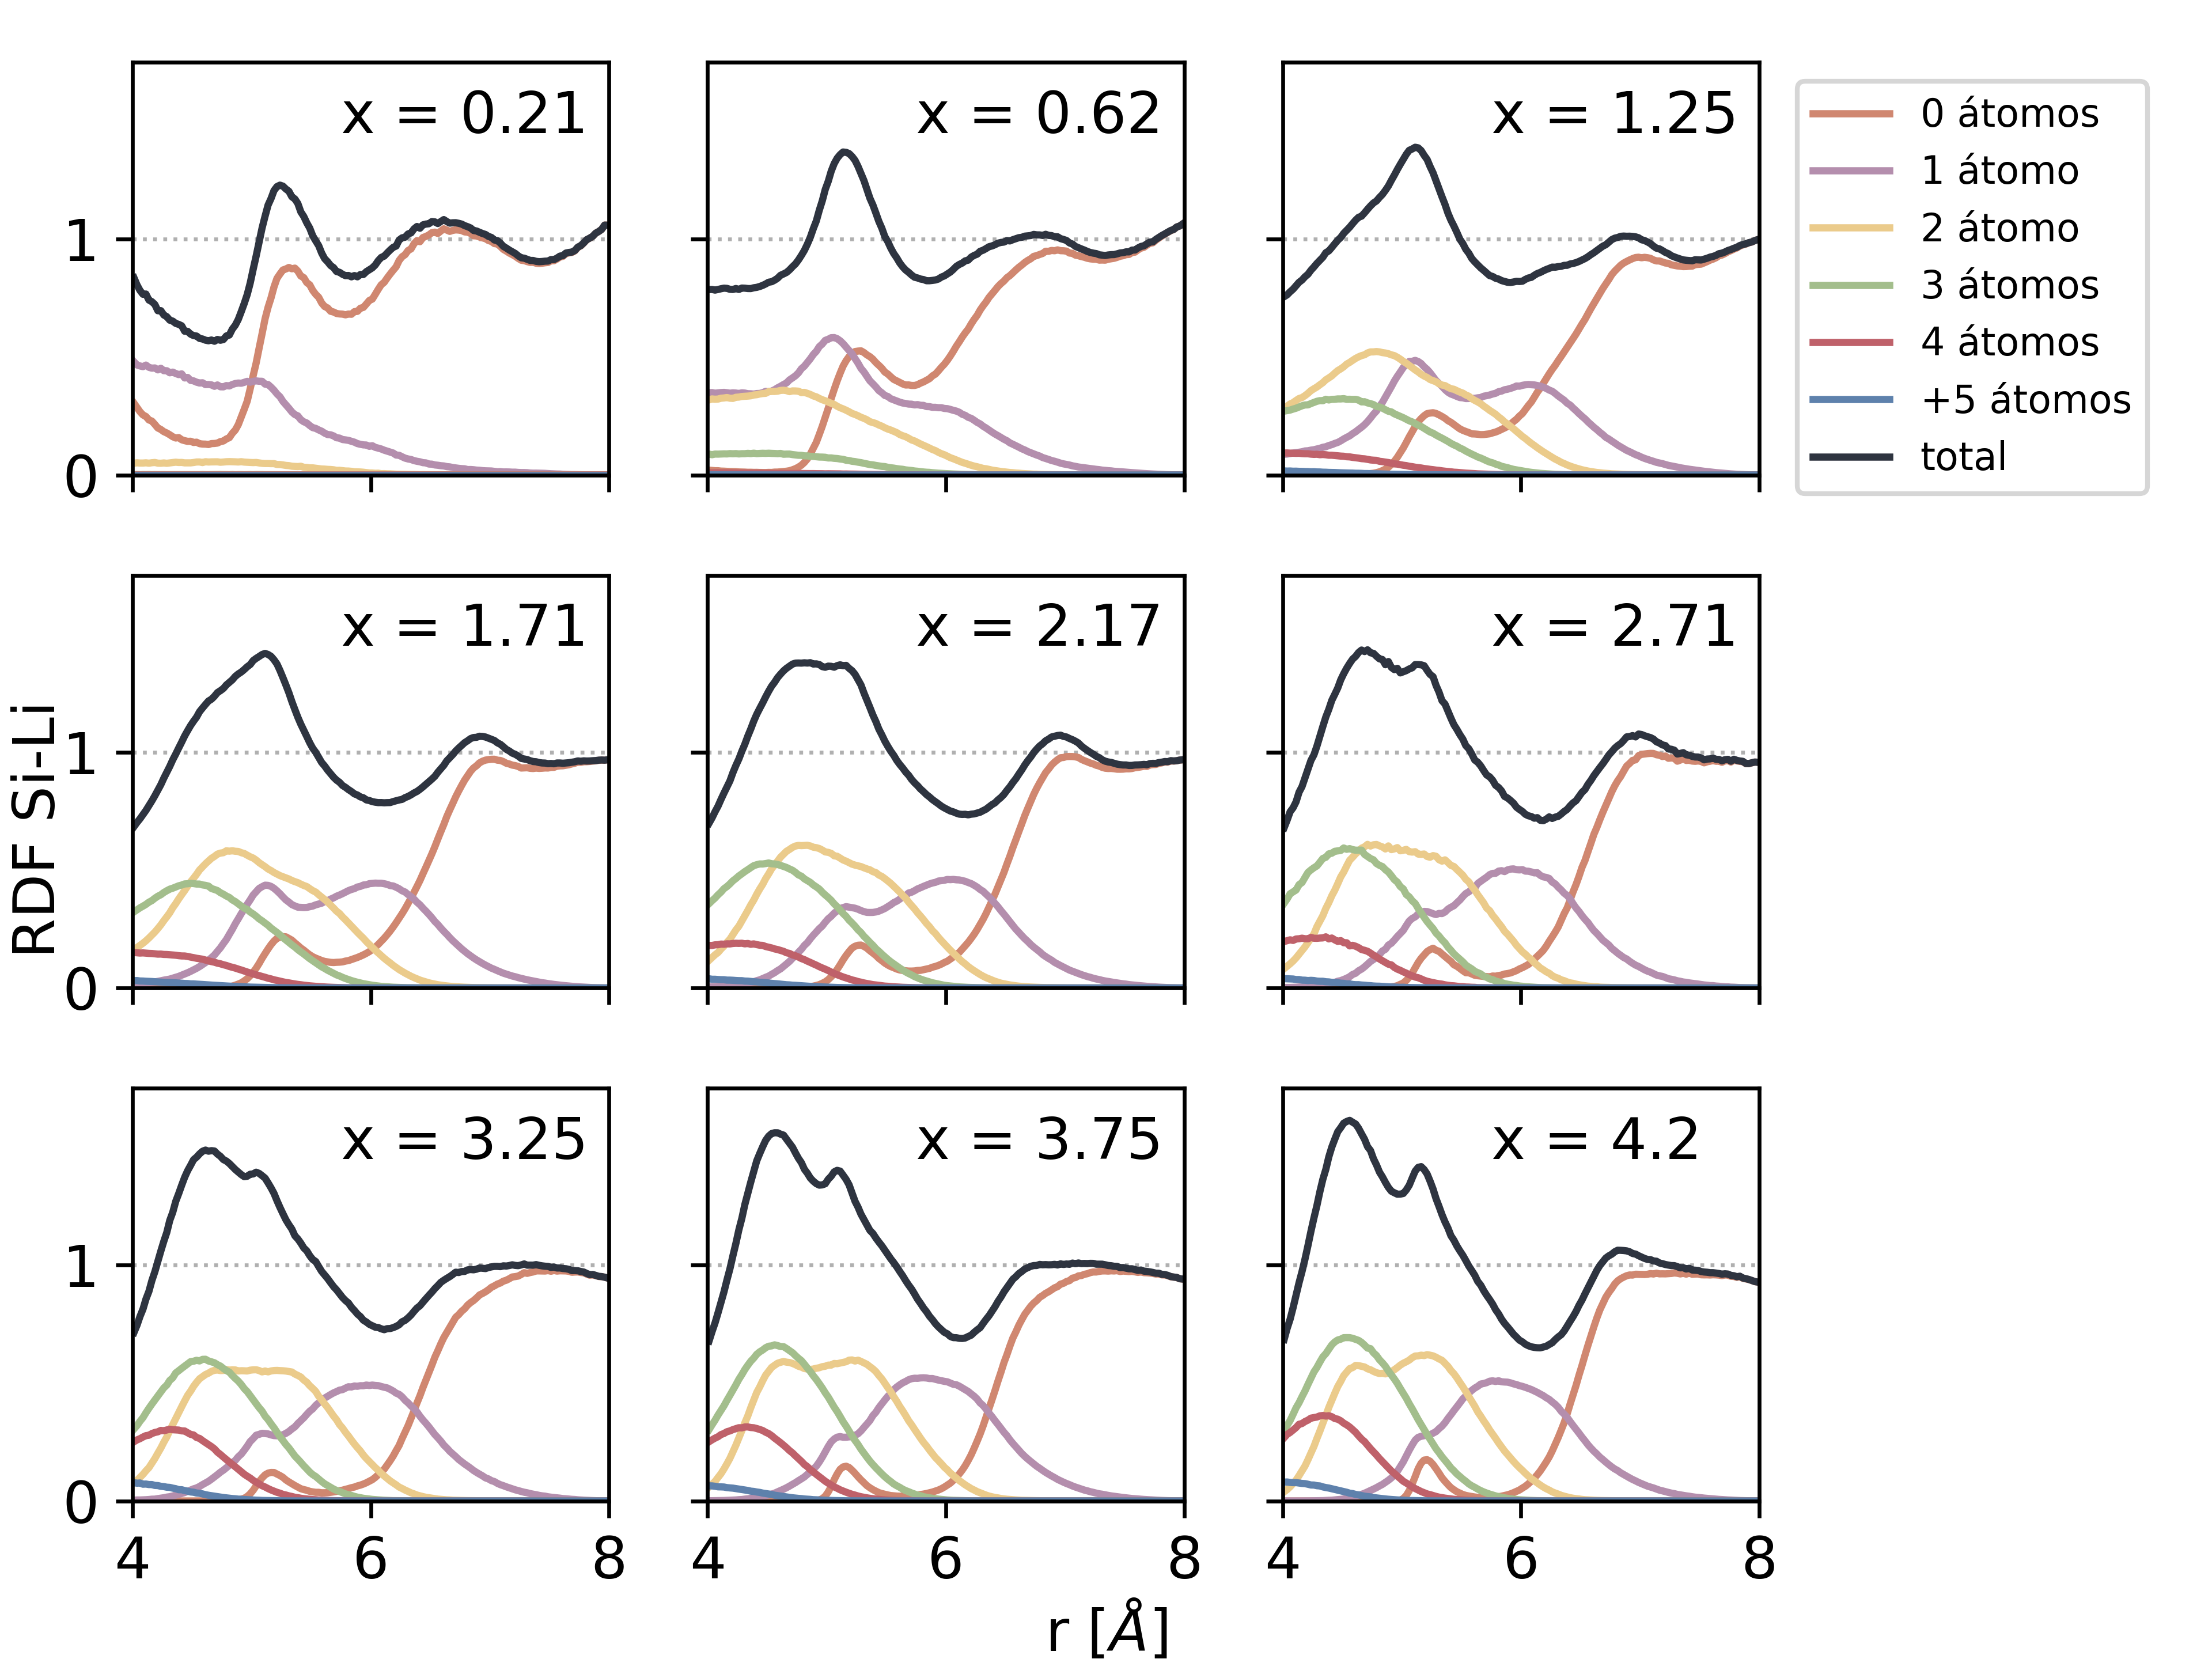
\includegraphics[width=\textwidth]{caracterizacion/interconexiones.png}
    \caption{Interconexiones de los segundos vecinos más cercanos de Li con un 
    átomo central de Si para cada valor de $x$ en Li$_x$Si considerado. El número 
    de primeros vecinos más cercanos que conectan a los segundos vecinos más 
    cercanos con el átomo central de Si se indica en el recuadro de las figuras. 
    Además de la RDF$_{Si-Li}$ total, se grafica cada una de las contribuciones 
    de los diferentes tipos de interconexiones posibles.}
    \label{fig:interconexiones}
\end{figure}

Mientras que el comportamiento presentado en la figura \ref{fig:interconexiones}
es más bien complejo, pueden establecerse tendencias generales que ayudan a 
entender mejor que es lo que sucede. Si se divide la RDF$_{Si-Li}$ en dos 
contribuciones de segundos vecinos, la primera de ellas, que se encuentra a una
distancia entre 4.0 \AA\ y 5.0 \AA, se puede atribuir a los átomos que tienen dos 
o más interconexiones de Li, mientras que la segunda de ellas, entre 5.0 \AA\ y
5.6 \AA, se corresponde con los átomos que tiene una o ninguna interconexión de 
Li. Utilizando esta clasificación, se muestra en la figura 
\ref{fig:interconexiones-areas} la fracción del área que representa cada una de
estas categorías en función de la concentración de litio.
\begin{figure}[th]
    \centering
    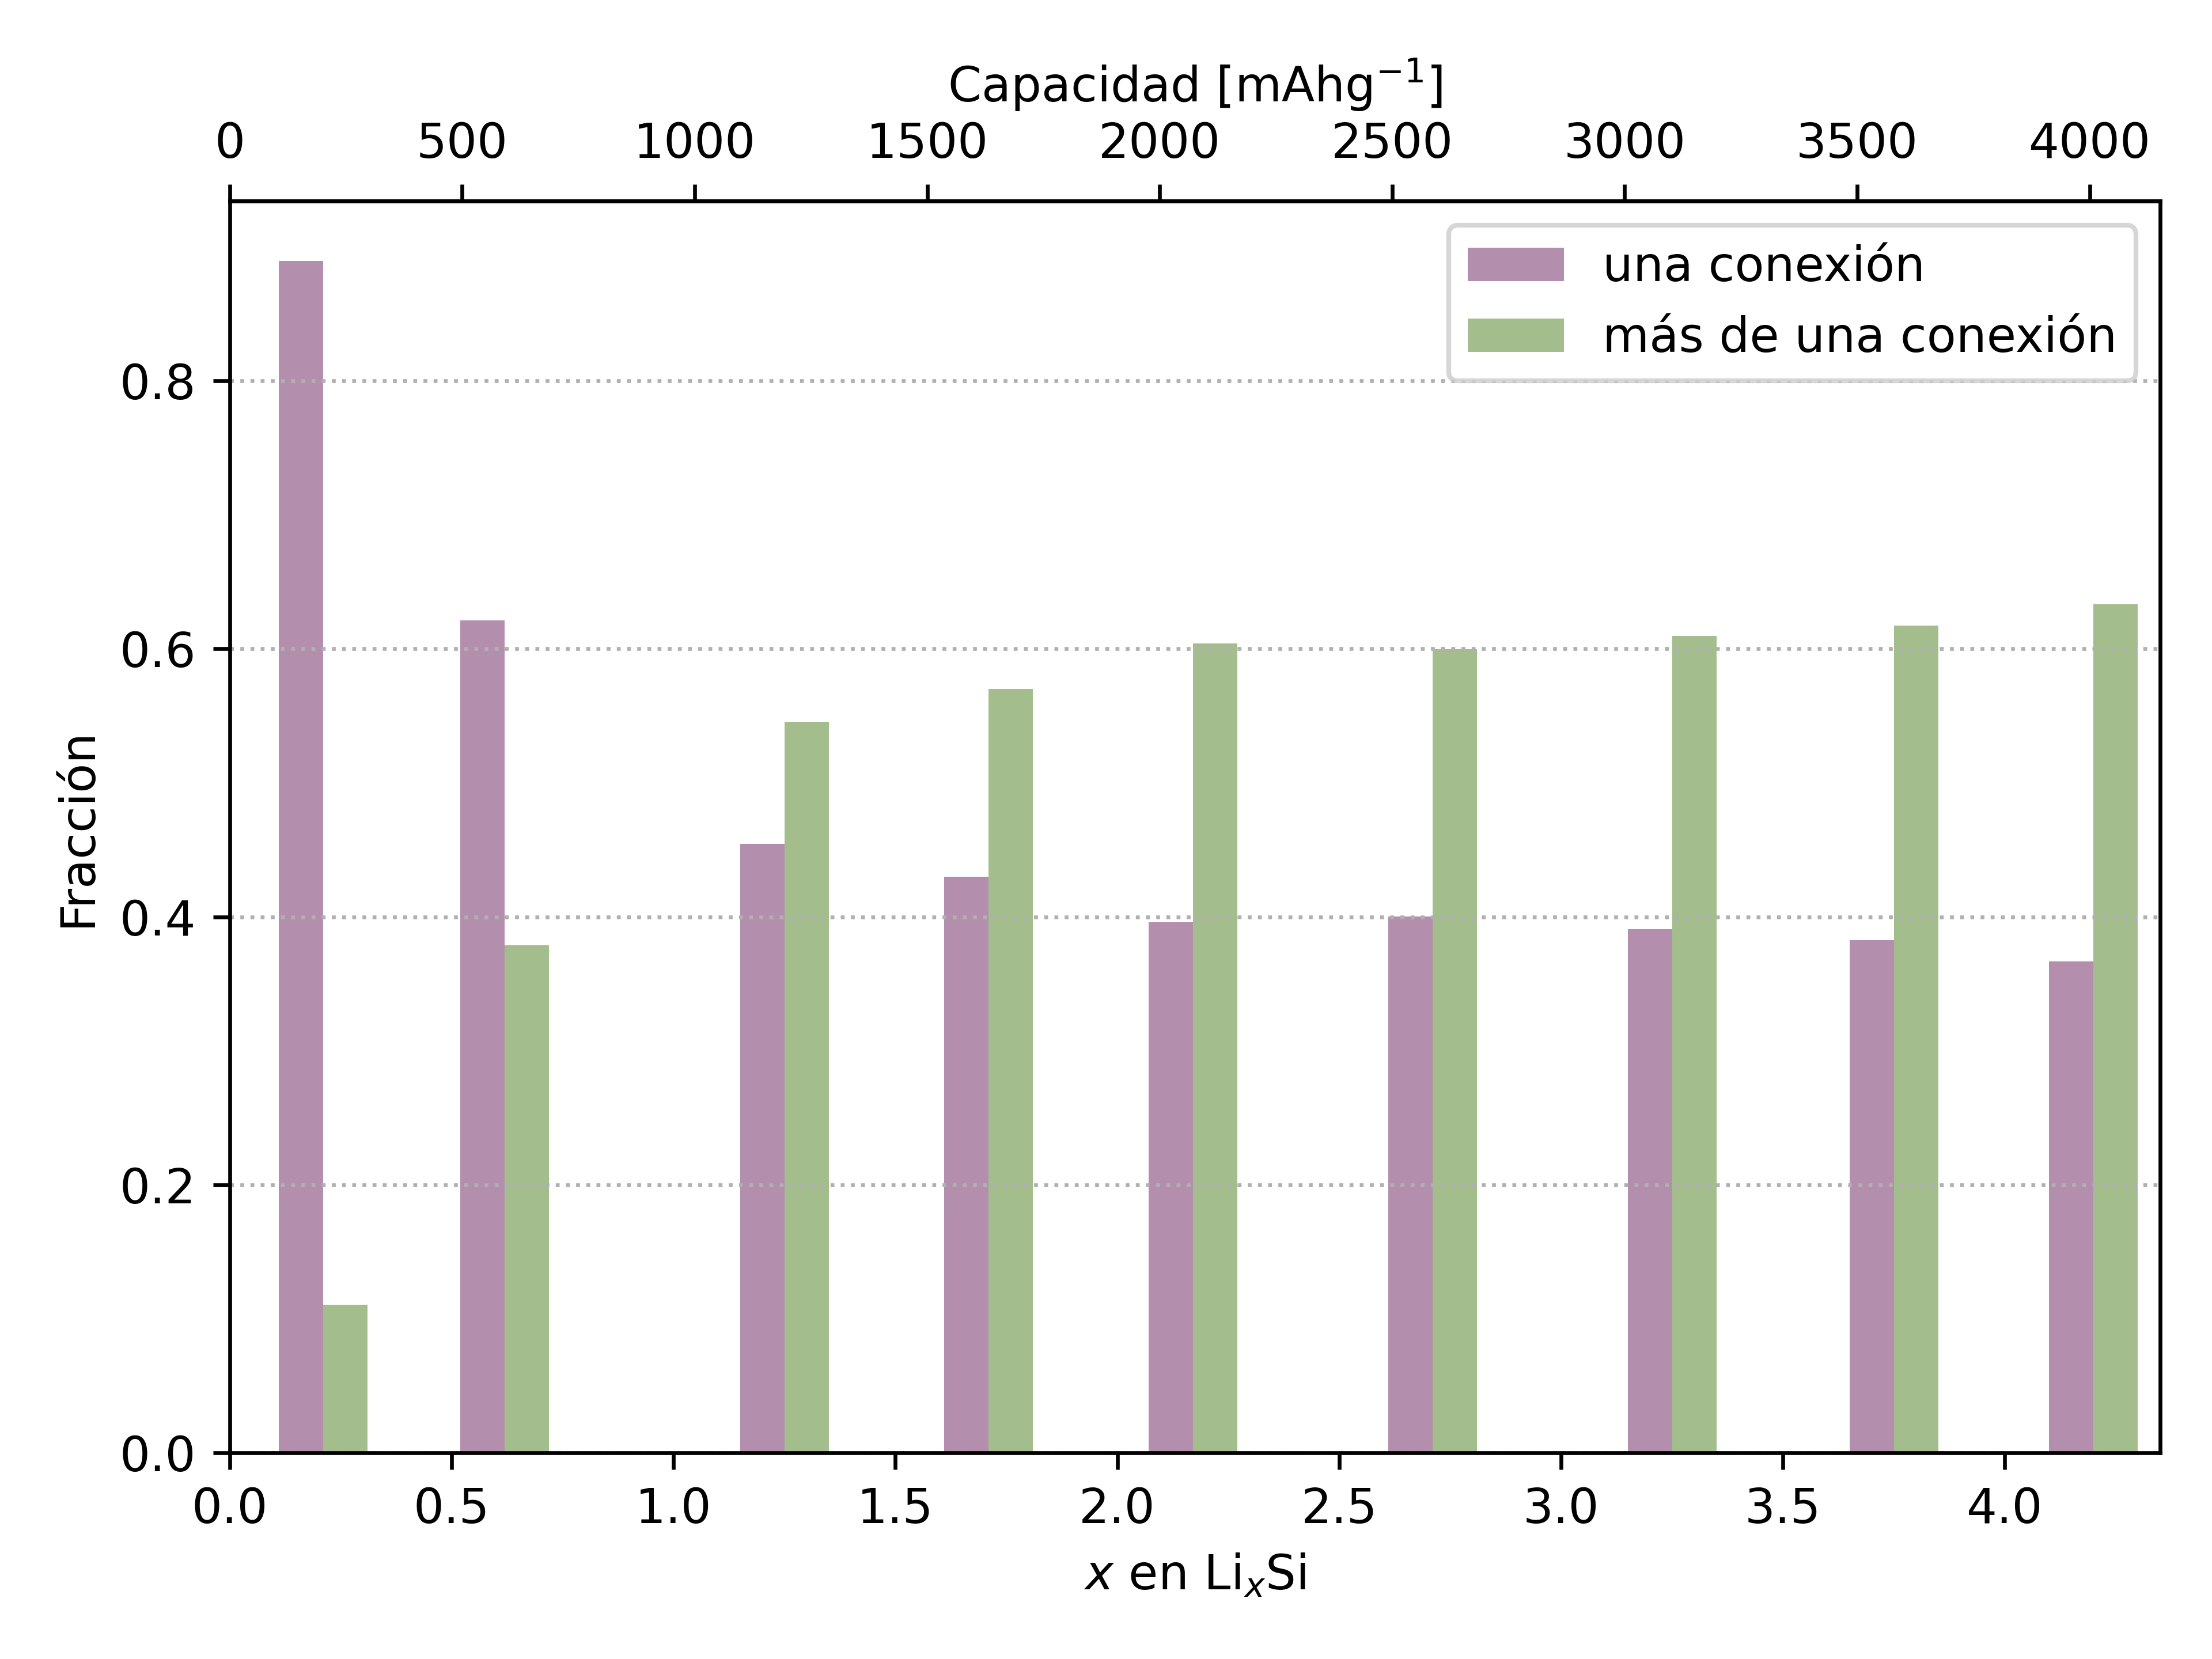
\includegraphics[width=0.8\textwidth]{caracterizacion/interconexiones-areas.png}
    \caption{Evolución con la concentración de la fracción que representa cada
    categoría de interconexiones de Li al área total del segundo pico de la 
    RDF$_{Si-Li}$.}
    \label{fig:interconexiones-areas}
\end{figure}

\subsection{Orden de corto alcance}

El término orden de corto alcance (SRO, de sus siglas en inglés 
\textit{short-range order}) se utiliza para denotar el ordenamiento de los átomos
que rodean a uno específico en una cáscara. Del mismo modo, el término 
\textit{clustering} se ha se ha definido como la tendencia de los átomos 
similares a estar cerca unos de otros. Ambos conceptos se refieren a un orden 
estructural entre átomos vecinos, pero no son necesariamente persistentes a 
distancias más largas. Warren ~\cite{warren69} y Cowley ~\cite{cowley1950} 
definieron un parámetro (WCP) para caracterizar estos tipos de ordenamientos de 
la siguiente manera:
\begin{equation}
    WCP = 1 - \frac{p_{A-B}}{m_B} = 1 - \frac{p_{B-A}}{m_A},
\end{equation}
donde $p_{A-B}(p_{B-A})$ es la probabilidad de tener un átomo de tipo B(A) como
vecino de un átomo de tipo A(B) y $m_B(m_A)$ es la concentración global de átomos
B(A), expresadas en fracciones molares. La igualdad, en ambas definiciones 
posibles del WCP, viene del hecho de que la probabilidad de encontrar a un átomo 
de tipo A como vecino de un átomo de tipo B es igual a la de tener un átomo de 
tipo B como vecino de un átomo de tipo A, esto es $m_A p_{A-B} = m_B p_{B-A}$.

Los valores que se obtienen de utilizar el parámetro WCP en sistemas del tipo
A$_x$B indica una aleatoriedad completa si es igual a cero, preferencia por 
átomos de distinto tipo si $WCP < 0$ y preferencia por átomos del mismo tipo si 
$WCP > 0$. Aunque este parámetro permite un análisis cuantitativo notable, sólo
se define para sistemas cristalinos en los que cada átomo tiene el mismo número
de vecinos. ~\cite{warren69}

A continuación se extiende esta idea para definir un nuevo parámetro, 
$\theta_{A-B}$, que es adecuado para caracterizar estructuras amorfas, de la 
siguiente manera:
\begin{equation}
    \theta_{A-B} = \ln \left( \frac{C_{A-B}}{C_{Bulk}} \right),
\end{equation}
donde A indica la naturaleza del átomo que se considera como central y B el tipo
de átomo que se considera como vecino, equivalente a la definición de WCP. En
este caso, la relación entre la concentración local y la concentración global se 
calcula a partir de la integración de la distribución radial de a pares parcial,
$g_{A-B}(r)$, en una esfera al rededor del átomo central,
\begin{equation}
    \frac{C_{A-B}}{C_{Bulk}} = \frac{1}{V(r_{cut})} \int_0^{r_{cut}} g_{A-B}(r) dV,
\end{equation}
donde $r_{cut}$ y $V(r_{cut})$ son el radio de corte y el volumen de la esfera 
considerada. Ya que en $g_{A-B}(r)$ no hay dependencia angular, $dV$ puede 
escribirse como $4 \pi r^2 dr$. Esta cantidad puede pensarse como la 
concentración promedio dentro de la esfera relativa a la del material 
\textit{bulk}. Así, de forma análoga al parámetro de WCP, $\theta_{A-B}$ indica 
la tendencia SRO o el \textit{clustering} para cualquier tipo de átomo dado.
Si $\theta$ es positivo, indica una acumulación de átomos relativa al 
\textit{bulk}, mientras que si es negativo indica una disminución. Si es igual a 
cero se tiene una aleatoriedad completa. Este nuevo parámetro también satisface 
la relación $\theta_{A-B} = \theta_{B-A}$ de la misma manera que se discutió para
el parámetro de WCP, ya que por definición $g_{A-B}(r) = g_{B-A}(r)$. Por lo cual 
se tiene que el parámetro $\theta_{A-B}$ da información similar a la que provee 
el WCP, pero además es aplicable a sistemas amorfos.

La figura \ref{fig:sro} muestra la variación del parámetro $\theta$ en función 
de la concentración de Li. Hay tres posibilidades para el análisis de $\theta$ en
sistemas de Li$_x$Si ($\theta_{Li-Li}$, $\theta_{Si-Si}$ y $\theta_{Si-Li}$), ya
que $\theta_{Si-Li} = \theta_{Li-Si}$. Para todos los casos se consideraron los
mismos radios de corte que en los cálculos del número de coordinación, luego del
primer pico de la RDF correspondiente.
\begin{figure}[th]
    \centering
    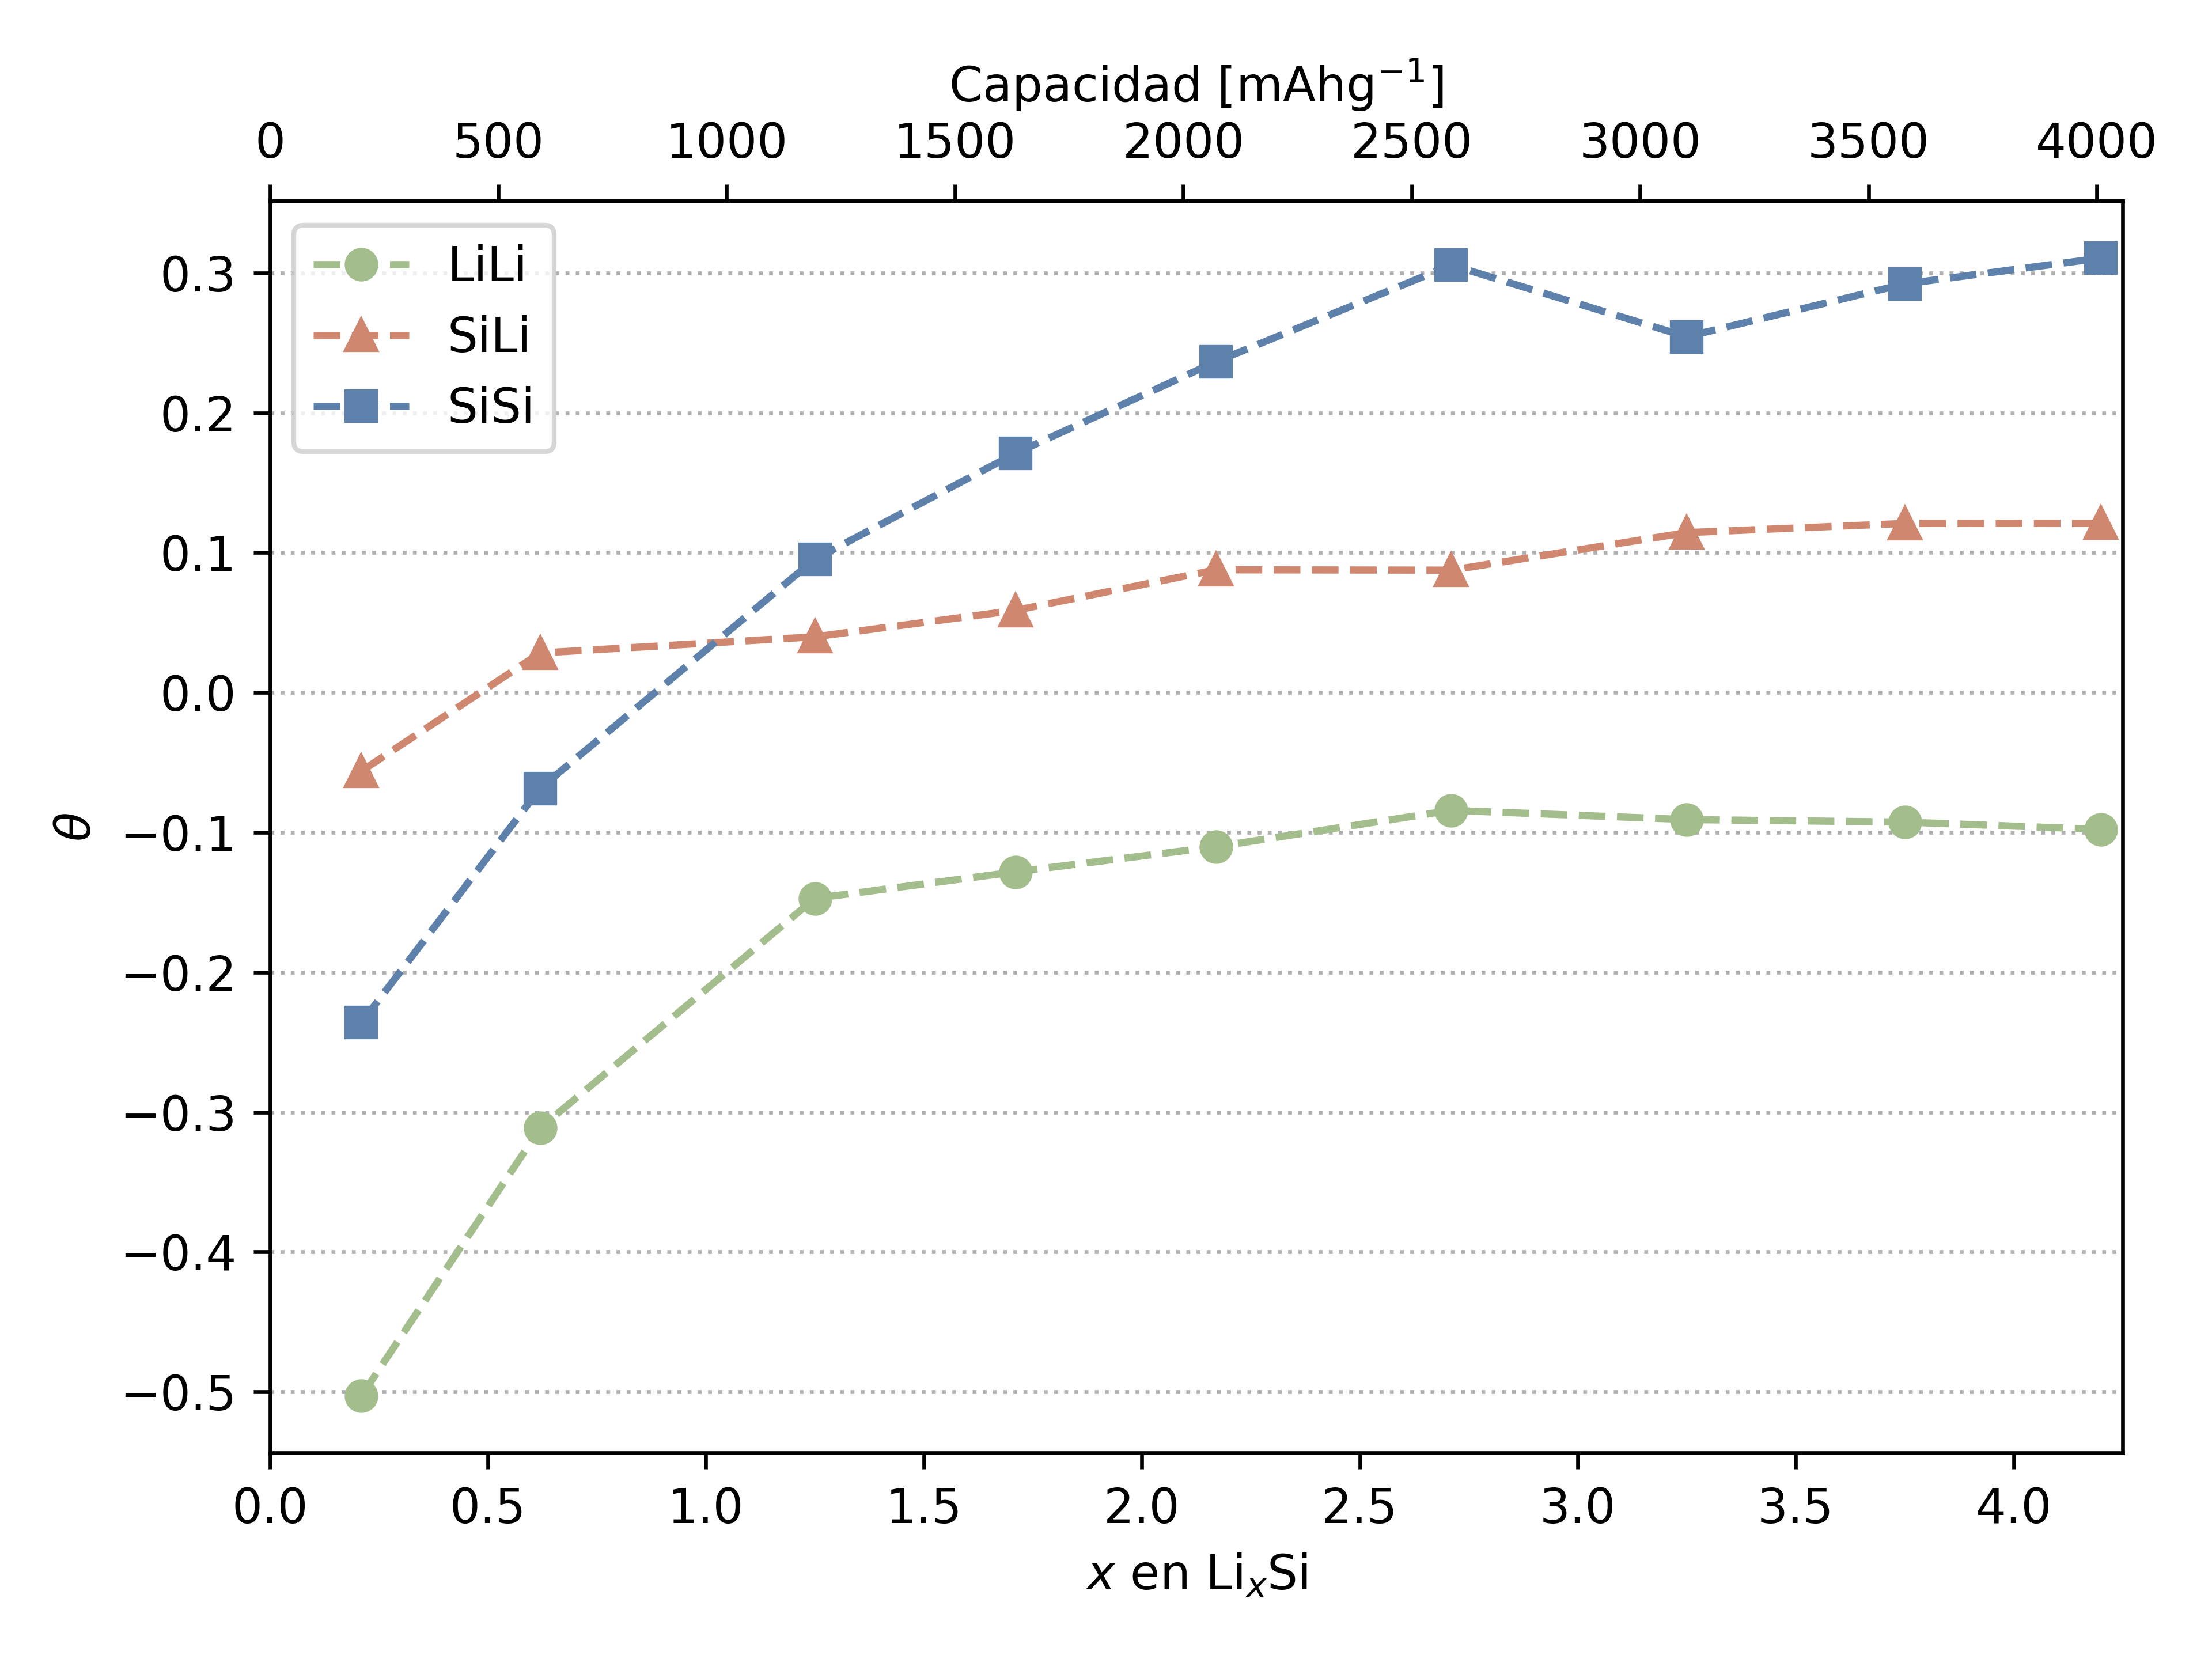
\includegraphics[width=0.8\textwidth]{caracterizacion/sro.png}
    \caption{Parámetros $\theta_{Li-Li}$, $\theta_{Si-Li}$ y $\theta_{Si-Si}$ 
    en función de la concentración de Li. El primer subíndice indica el tipo de
    átomo que se considera como central mientras que el segundo es el vecino. El
    radio de corte se eligió luego del primer pico de la RDF correspondiente.}
    \label{fig:sro}
\end{figure}

Como tendencia general, puede notarse que todos los valores de $\theta$ aumentan
cuando crece la cantidad de litio en el sistema, $x$, y que se estabiliza para 
valores grandes de $x$. Este comportamiento monótono y la disminución en la 
pendiente para concentraciones altas está correlacionado con el comportamiento
presentado en el análisis de los números de coordinación.

En el caso de $\theta_{Si-Si}$, alcanza un valor positivo aproximadamente 
constante para $x > 2.5$, mostrando una correlación fuerte con la presencia de 
cadenas lineales de Si, previamente discutidas y observadas en la figura 
\ref{fig:amorfas}. Aunque la presencia de estas cadenas se puede inferir a partir
de los valores de los CN en $x$ altos, $\theta$ es más sensible al SRO, ya que
está normalizado por la concentración global. Esta propiedad de $\theta$ permite
un análisis más claro incluso si las cadenas están interactuando entre sí, como
es el caso para concentraciones bajas de litio.

$\theta_{Si-Li}$ presenta variaciones pequeñas y un valor positivo para todo 
$x > 0.5$, mostrando una acumulación constante de Li al rededor del Si, o, 
análogamente, una acumulación de Si alrededor del Li. Este comportamiento se le 
puede atribuir a la interacción atractiva fuerte entre Si-Li. En el caso de 
$\theta_{Li-Li}$, este parámetro es siempre negativo, lo que indica una 
interacción débil Li-Li y la correspondiente disminución de vecinos Li-Li. Por
último, el parámetro $\theta_{Si-Si}$ tiene un valor negativo para $x < 1.0$, 
sugiriendo que la presencia de concentraciones bajas de litio tiende a separar 
los átomos de silicio entre sí. Sin embargo, $\theta_{Si-Si}$ se vuelve positivo
para $x > 1.0$, implicando una acumulación de vecinos de Si sobre átomos de Si, 
relativo a la concentración global. Esto se debe a la formación de estructuras 
Si-Si. Para $x > 2.5$ puede observarse un valor constante de 
$\theta_{Si-Si} \approx 0.3$, revelando la formación de estructuras estables de 
Si-Si dadas por las cadenas previamente mencionadas.


\section{Conclusiones del capítulo}

Con el fin de emular las estructuras amorfas encontradas en muchos experimentos 
electroquímicos, en este capítulo se generaron estructuras desordenadas de 
aleaciones de Li$_x$Si para varios valores de $x$ utilizando un algoritmo de 
dinámica acelerada y un campo de fuerzas reactivo. La exploración acelerada de 
mínimos locales (AELM) permitió la caracterización de una amplia gama de 
estructuras amorfas. El cambio de volumen de las estructuras litiadas en relación 
con el Si está en concordancia con los resultados experimentales de AFM. Las
energías de las estructuras obtenidas representan bien el comportamiento 
electroquímico de la curva de potencial en función de la concentración de Li. Se 
analizó la función de distribución radial de a pares para los diferentes tipos de 
pares atómicos y se dilucidó la estructura compleja del segundo pico del RDF 
Si-Li mediante un análisis de interconexión de clusters. Además, haciendo un 
análisis de la formación de clústeres en función del radio de corte, se demostró 
que las estructuras amorfas no presentan diferentes enlaces de Si ni átomos de Si 
aislados. En su lugar, se encontró que el sistema se comporta como una red amorfa. 
Estudiando los números de coordinación de primeros y segundos vecinos para las 
diferentes concentraciones, se mostró que esta red amorfa mantiene las conexiones 
tetraédricas para bajas concentraciones de Li y que tiende a formar cadenas para 
altas concentraciones de Li. Por último, la definición de un nuevo parámetro 
permitió determinar el orden de corto alcance de las estructuras amorfas, definido 
por interacciones débiles Li-Li y fuertes Li-Si y Si-Si. El método propuesto AELM 
resulta ser un método rápido y eficaz para obtener mínimos energéticamente 
relevantes. Se hizo una analogía con el templado simulado múltiple. Un análisis 
detallado de la eficiencia de AELM en comparación con otros métodos eficientes 
como el templado simulado múltiple o los métodos de Monte Carlo es una motivación 
para trabajos futuros.